\pdfoutput=1

\documentclass[11pt]{article}

\usepackage{EMNLP2023}

\usepackage{times}
\usepackage{latexsym}

\usepackage[T1]{fontenc}

\usepackage[utf8]{inputenc}

\usepackage{microtype}

\usepackage{inconsolata}


\usepackage{times}
\usepackage{latexsym}
\usepackage{graphicx}
\usepackage{amsmath}
\usepackage{amssymb}
\usepackage{booktabs}
\usepackage{textcomp}
\usepackage{multirow}
\usepackage{array}
\usepackage{bbm}
\usepackage{tabularx, booktabs}
\newcolumntype{Y}{>{\centering\arraybackslash}X}
\newcolumntype{L}{>{\arraybackslash}X}
\renewcommand\tabularxcolumn[1]{m{#1}}
\usepackage{inconsolata}
\usepackage{tablefootnote}
\usepackage{subcaption}

\usepackage[T1]{fontenc}

\usepackage[utf8]{inputenc}

\usepackage{microtype}

\usepackage{xparse}
\setlength{\belowcaptionskip}{-5pt}

\definecolor{bluepigment}{rgb}{0.2, 0.2, 0.6}
\definecolor{emerald}{rgb}{0.31, 0.78, 0.47}
\definecolor{orange}{rgb}{0.91, 0.41, 0.17}
\newcommand{\ours}{CEDAR}
\newcommand{\datasetname}{\textsc{GLEN}}
\newcommand{\tabincell}[2]{\begin{tabular}{@{}#1@{}}#2\end{tabular}}


\title{GLEN: General-Purpose Event Detection for Thousands of Types} 


\author{Qiusi Zhan$^1$*, Sha Li$^1$*, Kathryn Conger$^2$, Martha Palmer$^2$, Heng Ji$^1$, Jiawei Han$^1$ \\
  $^1$University of Illinois Urbana-Champaign \\
  $^2$University of Colorado Boulder \\
  \texttt{\{qiusiz2, shal2, hengji, hanj\}@illinois.edu} \\
  \texttt{\{kathryn.conger, martha.palmer\}@colorado.edu} 
  }

\begin{document}
\maketitle
\begin{abstract}
\IEEEtitleabstractindextext{%
\begin{abstract}
Vision transformer (ViT) expands the success of transformer models from sequential data to images. The model decomposes an image into many smaller patches and arranges them into a sequence. Multi-head self-attentions are then applied to the sequence to learn the attention between patches. 
Despite many successful interpretations of transformers on sequential data, little effort has been devoted to the interpretation of ViTs, and many questions remain unanswered. For example, among the numerous attention heads, which one is more important? 
How strong are individual patches attending to their spatial neighbors in different heads? What attention patterns have individual heads learned? 
In this work, we answer these questions through a visual analytics approach. Specifically, we first identify \textbf{\textit{what}} heads are more important in ViTs by introducing multiple pruning-based metrics. 
Then, we profile the spatial distribution of attention strengths between patches inside individual heads, as well as the trend of attention strengths across attention layers.
Third, using an autoencoder-based learning solution, we summarize all possible attention patterns that individual heads could learn. Examining the attention strengths and patterns of the important heads, we answer \textbf{\textit{why}} they are important. 
Through concrete case studies with experienced deep learning experts on multiple ViTs, we validate the effectiveness of our solution that deepens the understanding of ViTs from \textit{head importance}, \textit{head attention strength}, and \textit{head attention pattern}.
\end{abstract}

% Note that keywords are not normally used for peerreview papers.
\begin{IEEEkeywords}
Vision transformer, multi-head self-attention, deep learning, explainable artificial intelligence, visual analytics.
\end{IEEEkeywords}}
\end{abstract}
\section{Introduction}
Graph neural networks (GNNs) have undergone rapid development and become increasingly popular for learning graph data \cite{welling2016semi, velivckovic2017graph, xu2018powerful}.
GNNs are usually trained in an end-to-end manner while getting enough labeled data is arduously expensive and sometimes even impractical to access. This motivates some recent advances in pre-training GNNs ~\cite{hu2019strategies,Hu2020GPTGNNGP,Qiu2020GCCGC,Lu2021LearningTP}. 
The key insight of pre-training GNNs is to learn transferable knowledge from a collection of unlabeled graph data, hoping that the learned knowledge can be easily adapted to downstream tasks.
In view of the great success of pre-training in other fields like computer vision and natural language processing~\cite{devlin2018bert,he2020momentum},  graph pre-training is {highly expected} to be an effective means to improve downstream performance.


\begin{figure}[t]
    \centering
    {\includegraphics[width=1\columnwidth]{figure/motivation.pdf}}
    \caption{Comparison of {existing methods} and {proposed W2PGNN} to answer \emph{when to pre-train} GNNs.}    
    \label{fig:example}
\end{figure}

However, the intuition that graph pre-trained model would ideally benefit the downstream is far from the truth in the area of graph pre-training.
Instead, graph pre-trained models can lead to \emph{negative transfer} on many downstream tasks, especially when the graphs used for pre-training are not necessarily from the same domain as the {downstream} data~\cite{hu2019strategies, Qiu2020GCCGC}.
For example, the closed triangles ($\vcenter{\hbox{\includegraphics[width=2.4ex,height=2.4ex]{figure/s2.pdf}}}$) and open triangles  ($\vcenter{\hbox{\includegraphics[width=2.4ex,height=2.4ex]{figure/s1.pdf}}}$) might yield different interpretations in molecular networks (unstable vs. stable in terms of chemical property) from those in social networks (stable vs. unstable in terms of social relationship); such distinct or reversed semantics does not contribute to transferability, and even exacerbates the problem of negative transfer.


To avoid the negative transfer, recent efforts focus on  \emph{what to pre-train} and \emph{how to pre-train},  \emph{i.e.}, design/adopt graph pre-training models with a variety of self-supervised tasks to capture different patterns~\cite{Qiu2020GCCGC,you2020graph,Lu2021LearningTP} and fine-tuning strategies to enhance downstream performance~\cite{Hu2019PreTrainingGN,Han2021AdaptiveTL,Zhang2022FineTuningGN,Xia2022TowardsEA}.
However, there do exist some cases that no matter how advanced the pre-training/fine-tuning method is, the transferability from pre-training data to downstream data still cannot be guaranteed. This is because the underlying assumption of deep learning models is that the test data should share a similar distribution as the training data.
Therefore, it is a necessity to understand \emph{when to pre-train}, \emph{i.e.}, under what situations the ``graph pre-train and fine-tune'' paradigm should be adopted.

Towards the answer of when to pre-train GNNs, one straight-forward way illustrated in Figure~\ref{fig:example}(a) is to train and evaluate on all candidates of pre-training models and fine-tuning strategies, and then the resulting best downstream performance would tell us whether pre-training
% ``pre-train and fine-tune'' 
is a sensible choice. If there exist $l_1$ pre-training models and $l_2$ fine-tuning strategies,  such a process would be very costly as you should make $l_1 \times l_2$ ``pre-train and fine-tune'' attempts.
Another approach is to utilize graph metrics to measure the similarity between pre-training and downstream data, \emph{e.g.}, density, clustering coefficient and etc. However, it is a daunting task to enumerate all hand-engineered graph features or find the dominant features that influenced similarity.
Moreover, the graph metrics only measure the pair-wise similarity between two graphs, which cannot be directly and accurately applied to the practical scenario where pre-training data contains multiple graphs.


In this paper, we propose a W2PGNN framework to answer
\emph{\underline{w}hen \underline{to} \underline{p}re-train \underline{GNN}s from a graph data generation perspective}.
% aim to address the problem of when to pre-train GNNs 
The high-level idea is that instead of performing effortful graph pre-training/fine-tuning or making comparisons between the pre-training and downstream data, we study the complex generative mechanism from the pre-training data to the downstream data (Figure~\ref{fig:example}(b)).
We say that downstream data can benefit from pre-training data (\emph{i.e.}, has high feasibility of performing pre-training), 
if it can be generated with high probability by a graph generator that summarizes the topological characteristic of pre-training data.



The major challenge is how to obtain an appropriate graph generator, hoping that it not only inherits the transferable topological patterns of the pre-training data, but also is endowed with the ability to generate feasible downstream graphs.
To tackle the challenge, we propose to design a graph generator based on graphons.
We first fit the pre-training graphs into different graphons to construct a \emph{graphon basis}, where each graphon (\emph{i.e.}, element of the graphon basis) identifies a collection of graphs that share common transferable patterns. We then define a \emph{graph generator} as {a convex combination of elements in a graphon basis}, which serves as a comprehensive and representative summary of pre-training data.  All of these possible generators constitute the \emph{generator space}, from which graphs generated form the solution space for the downstream data that can benefit from pre-training.

Accordingly, the feasibility of performing pre-training can be measured as the highest probability of downstream data being generated from any graph generator in the generator space, which can be formulated as an optimization problem.
However, this problem is still difficult to solve due to the large search space of graphon basis. We propose to reduce the search space to three candidates of graphon basis, \emph{i.e.,} topological graphon basis, domain graphon basis, and integrated graphon basis, to mimic different {generation mechanisms} from pre-training to downstream data. Built upon the reduced search space, the feasibility can be approximated efficiently.





Our major contributions are concluded as follows:
\begin{itemize}[leftmargin=*,topsep=0pt]
\item \textbf{Problem and method.} To the best of our knowledge, we are the first work to study the problem of when to pre-train GNNs. We propose a W2PGNN framework
to answer the question from a data generation perspective, which tells us the feasibility of performing graph pre-training before conducting effortful pre-training and fine-tuning.




\item \textbf{Broad applications.}
W2PGNN provides several practical applications: (1) provide the application scope of a graph pre-trained model, (2) measure the feasibility of performing pre-training for a downstream data
and (3) choose the pre-training data so as to maximize downstream performance with limited resources.


\item \textbf{Theory and Experiment.} 
We theoretically and empirically justify the effectiveness of W2PGNN.
Extensive experiments {on real-world graph datasets from multiple domains} show that the proposed method can provide an accurate estimation of pre-training feasibility and the selected pre-training data can benefit the downstream performance.


\end{itemize}


\subsection{Graph Property Prediction}

Graph neural networks (GNNs)~\citep{kipf2017semi,xu2018powerful} are commonly used for graph property prediction in chemistry and polymer informatics tasks~\citep{otsuka2011polyinfo,hu2020open,zhou2022jointly}.
However, it is hard to annotate enough labels in these domains. 
Recent work used \textit{self-supervised tasks} such as node attribute prediction and graph structure prediction~\citep{hu2019strategies,you2021graph,kim2022graph} to pre-train architecture-fixed GNNs. \citet{sun2022does} observed that the existing methods might fail to transfer knowledge from unlabeled graph data. Flexible GNN architectures for downstream tasks would be desirable.

\textit{Graph data augmentation} (GDA) methods do not restrict GNN architecture choices to improve prediction accuracy~\citep{trivedianalyzing,zhao2022learning,zhao2022graph,ding2022data}.
They learn to create new examples that preserve the properties of original graphs~\citep{liu2022local,liu2022graph,kong2022robust,han2022g,luo2022automated}.
However, they purely manipulate labeled examples and thus \textit{cannot utilize the knowledge in unlabeled graphs}.
Our \method combines the knowledge from the unlabeled dataset and the labeled task dataset. It creates label-preserved graph examples with the knowledge transferred from the unlabeled data. It allows the GNN models to have flexible architectures.

\subsection{Learning from Unlabeled Data}

\textit{Pre-training on self-supervised tasks} such as masked image modeling and autoregressive text generation is effective for large language and vision models~\citep{brown2020language,he2022masked}. However, the hand-crafted self-supervised tasks could hardly help models learn useful knowledge from unlabeled graphs \emph{due to the gap between these label-agnostic tasks and the downstream prediction tasks} towards drug discovery and material discovery~\citep{sun2021mocl,kim2022graph,inae2023motif}.
A universal self-supervised task to learn from the unlabeled graphs remains under-explored~\citep{sun2022does,trivedianalyzing}.

\textit{Semi-supervised learning} assumes that unlabeled and labeled data are from the same source~\citep{liu2023semi}. The learning objective in the latent space is usually mutual information maximization that encourages similarity between the representations of unlabeled and labeled graphs~\citep{sun2019infograph}. However, \textit{the distributions of the unlabeled and labeled data could be very different} due to the different types of sources~\citep{hu2019strategies}, leading to negative impacts on the property prediction on the labeled graphs.
\textit{Self-training}, as a specific type of semi-supervised learning method, selects the unlabeled graphs of confidently predictable labels and assigns pseudo-labels for them~\citep{lee2013pseudo,iscen2019label}. Many studies have explored improving uncertainty estimation~\citep{gal2016dropout,tagasovska2019single,amini2020deep} to help the model filter out noise for reliable pseudo-labels. Recently, pseudo-labels have been applied in imbalanced learning~\citep{liu2023semi} and representation learning~\citep{ghiasi2021multi}. However, self-training is restricted to confidently predictable labels and may ignore the huge number of any other unlabeled graphs~\citep{huang2022uncertainty}. Therefore, it cannot fully utilize the knowledge in the unlabeled graphs. 

In contrast, our \method employs a diffusion model to extract knowledge (as the diffusion and reverse processes) from \textit{all the unlabeled graphs}. \method represents the knowledge as task-specific labeled examples to augment the target dataset, instead of uninterpretable pre-trained model parameters. We note that self- or semi-supervised learning does not conflict with \method, and we leave their combinations for future work.

\subsection{Diffusion Models on Graphs}
Recent works have improved the diffusion models on graphs~\citep{niu2020permutation,jo2022score,vignac2022digress,kong2023autoregressive,chen2023efficient}. EDP-GNN~\citep{niu2020permutation} employed score matching for permutation-invariant graph data distribution. GDSS~\citep{jo2022score} extended the continuous-time framework [6] to model node-edge joint distribution. DiGress~\citep{vignac2022digress} used the transition matrix to preserve the discrete natures of the graph structure. GraphARM~\citep{kong2023autoregressive} introduced a node-absorbing autoregressive diffusion process. EDGE~\citep{chen2023efficient} focused on efficiently generating larger graphs. Instead of improving the generation performance of the diffusion model, our model builds on score-based diffusion models~\citep{jo2022score,song2020score} for predictive tasks, \ie, graph classification and graph regression. %
\section{The \datasetname\ Benchmark}



\begin{figure*}[!t]
\centering
\begin{subfigure}{.5\textwidth}
  \centering
  \includegraphics[width=\linewidth]{figures/event_distribution.png}
  \caption{}
  \label{fig:sub1}
\end{subfigure}%
\begin{subfigure}{.5\textwidth}
  \centering
  \includegraphics[width=\linewidth]{figures/glen_data_longtail_clear.pdf}
  \caption{}
  \label{fig:sub2}
\end{subfigure}
\caption{The event type distribution of GLEN. In the training set, instances associated with $N$ labels are weighted as $\frac{1}{N}$. Figure (a) illustrates the distribution of event types based on the number of instances. In figure (b), we show the top three most popular event types as well as randomly sampled types from the middle and tail of the distribution curve.} 
\label{fig:glen_data_longtail}
\end{figure*}
To build the \datasetname\ benchmark, we first build a general-purpose ontology based on the curated DWD Overlay and then create distantly-supervised training data based on the refined ontology (Section \ref{sec:ontology}). In order to evaluate our model, we also create a labeled development set and test set through crowdsourcing (Section \ref{sec:annotation}). 
\subsection{Event Ontology and Data}
\label{sec:ontology}
The DWD Overlay is an effort to align WikiData Qnodes to PropBank rolesets, their argument structures, and LDC tagsets. 
This mapping ensures that our ontology is a superset of the ontology used in ACE and ERE~\cite{song-etal-2015-light}. (See Section \ref{sec:data_analysis} for a detailed comparison of the ontology coverage.) 

To make this ontology more suitable for the event extraction task, we remove the Qnodes related to cognitive events that do not involve any physical state change such as \texttt{belief} and \texttt{doubt}. \footnote{This is in line with the scope of events as defined in previous ACE and ERE datasets.}
We also discovered that many rolesets such as \texttt{ill.01} were heavily reused across the ontology (mainly due to the inclusion of very fine-grained types), therefore we manually cleaned up the event types that were associated with these rolesets. 
We show some examples of removed Qnodes in Appendix Table \ref{tab:removed_nodes}.




\label{sec:data_cleaning}
Since the DWD Overlay is aligned with PropBank, we propose to reuse the existing PropBank annotations\footnote{\url{https://github.com/propbank/propbank-release}}. 
After the automatic mapping, each event mention in the dataset would be associated with one or more Qnodes, which leads to the \textbf{partial label} challenge when using this distantly-supervised data.
We then perform another round of data filtering based on the frequency of rolesets (details in Appendix \ref{sec:appendix_annotation}).
After these cleaning efforts, we used the annotation for 1,804 PropBank rolesets, which are mapped to a total of 3,465 event types. 

To make our data split more realistic and to preserve the document-level context, 
we split the dataset into train, development, and test sets based on documents using a ratio of 90/5/5. Note that although our test set is only 5\% of the full data, it is already similar in scale to the entire ACE05 dataset. 
For datasets such as OntoNotes and AMR that contain documents from multiple genres (newswire, broadcast, web blogs etc.), we perform stratified sampling to preserve the ratio between genres. 
The statistics of our dataset are listed in Table \ref{tab:data}. Compared with ACE05 and MAVEN, \datasetname\ utilizes a 20x larger ontology and 4x larger corpus. 

        

\begin{figure*}[!t]
    \centering
    \includegraphics[width=0.99\linewidth]{figures/xpo_ace_comparison_fig.pdf}
    \caption{
    A comparison between our ontology and that of ACE. 
    Our dataset offers broader coverage of events compared to ACE05, with diverse branches ranging from \texttt{sports\_competition} to \texttt{military\_operation}. 
    }
    \label{fig:xpo_ace_comparison}
\end{figure*}

\subsection{Data Annotation}
\label{sec:annotation} 
Instead of performing annotation from scratch, we formulate the annotation task as a multiple-choice question: the annotators are presented with the trigger word in context and asked to choose from the Qnodes that are mapped to the roleset. 


For the test set, we hired graduate students with linguistic knowledge to perform annotation.
For the development set, we screened Mechanical Turk workers that had high agreement with our in-house annotators and asked those who passed the screening to participate in the annotation. 
The weighted average kappa value for exact match on the test set (27 annotators), is 0.60, while for the dev set (981 annotators) is 0.37 over 5.2 options.  If we allow for a soft match for event types of different granularity, 
such as \texttt{trade} and \texttt{international\_trade},
the kappa value is 0.90 for the test set and 0.69 for the dev set.
For more details on the annotation interface, see Appendix \ref{sec:appendix_annotation}.



\subsection{Data Analysis}
\label{sec:data_analysis}
We first examine our event ontology by visualizing it as a hierarchy (as shown in Figure \ref{fig:xpo_ace_comparison}) with the parent-child relations taken from Wikidata (the \texttt{overlay\_parent} field in DWD Overlay).
Our ontology offers a wider range of diverse events, including those related to military, disaster, sports, social phenomena, chemicals, and other topics, indicating its novelty and potential usefulness.


We show the event type distribution in our dataset in 
Figure \ref{fig:glen_data_longtail}. 
Our type distribution closely mirrors real-world event distributions. The distribution exhibits frequent events such as \texttt{come} and \texttt{use}, along with a long tail of rare events such as \texttt{defect} and \texttt{impiety}. 
In terms of type diversity, for ACE, the single most popular event type \texttt{attack} accounts for 28.8\% of the instances and the top-10 event types account for 79.4\% of the data. Our type distribution is much less skewed with the top-10 events composing 8.3\% of the data. 

\begin{figure}[!t]
    \centering
    \includegraphics[width=0.99\linewidth]{figures/pos_blue.pdf}
    \caption{
    The Part-of-Speech distribution of trigger words for events in GLEN. Multiple POS tags mean that the trigger has multiple words. 
    }
    \label{fig:pos_dis}
\end{figure}
Figure \ref{fig:pos_dis} illustrates the part-of-speech distribution of trigger words in our dataset\footnote{We use universal POS tagging tools from \url{https://www.nltk.org/}. }. Over 96\% of trigger words are verbs or nouns, which is similar to that of 94\% in MAVEN and 90\% in ACE2005. In addition, 0.6\% of the triggers are multi-word phrases. 




\vspace{-2mm}
\section{Proposed Framework} \label{method}
\vspace{-2mm}

\begin{figure}[!tbp]
\centering

\includegraphics[width=12cm]{figure/teaser.pdf}
\caption{Illustration of the whole workflow. (a) shows how hypergraph information bottleneck utilised to optimize the representation $Z$ to capture the minimal sufficient information within the input data $D=(G,I)$ to predict the MCI conversion label $Y$. (b) is the overall workflow integrating HGIB into the hypergraph neural network. HGNNP is a kind of hypergraph convolutional layer.}
\label{teaser}

\end{figure}

This section presents a detailed description of the crucial components of our proposed framework. Firstly, we elucidate the process of constructing the hypergraph from a given set of multi-modal data, and we delve into the specifics of the hypergraph convolution definition. Secondly, we explicate the fundamental principle of information bottleneck and integrate it into hypergraph neural networks.
The overview of the proposed method is illustrated in Fig.~\ref{teaser}.

% Introduction why using hypergraph for mult-modality learning + HGIB



% \Angie{to be updated}



\smallskip
\subsection{Hypergraph Modelling and Hypergraph Convolution}

To overcome the
challenges associated with multi-modality data ($I_1, I_2, ..., I_m$), we leverage a hypergraph
structure $G$ to represent the multi-modal features ($X_1, X_2, ..., X_m$) extracted from backbones. Subsequently, we employ a hypergraph neural network to predict MCI conversion.

% The main purpose of the proposed framework is to optimally balance the expressiveness and robustness of the learned representation of hypergraph structure data for accurate MCI conversion prediction.
% 
%Hypergraph is general framework to incorporate with multi-modality data which is common strategy for AD diagnosis.
% 
% To encourage the minimal and sufficient representation learning, we introduce  information bottleneck by applying this principle to hypergraph neural networks.
% 
%We will first elaborate hypergraph modelling and hypergraph convolution operation and then introduce the hypergraph information bottleneck.

\medskip
\noindent
\textbf{Hypergraph representation learning.}
We consider an undirected attributed hypergraph $G = (V, E, \textbf{H})$ with a vertex set $V$, a hyperedge set $E$, and an adjacency matrix $\textbf{H} \in \mathbb{R}^{|V| \times |E|}$ for hyperedge weight. 
% 
Each vertex in our hypergraph structure corresponds to a patient, while each hyperedge represents the relationship between a subset of vertices. Unlike in a graph structure, where an edge connects only two vertices, a hyperedge in a hypergraph connects multiple vertices, enabling the representation of higher-order relationships. This feature facilitates the grouping of subsets of vertices with common features or properties, enhancing the ability of the hypergraph to model complex relationships within the data.
% 
In our hypergraph structure, each vertex corresponds to a patient and each hyperedge represents the relationship between a subset of the vertices. Unlike in a graph structure, a hyperedge in a hypergraph connects multiple vertices instead of just two, allowing for the representation of higher-order relationships. This can be seen as the hyperedges grouping together subsets of vertices that have common features or properties.
% 
Specifically, the hyperedge weight between vertex $v$ and hyperedge $e$ can be defined as 
$h_{v,e}= 
\left\{ 
    \begin{array}{lc}
        1& \text{if} \  v \in e \\
        0& \text{otherwise}
    \end{array}
\right.
$.
Moreover, we denote the vertex attributes as $X$, which can be seen as a feature embedding. The input data can be represented as $D=(G, X)$. In the multi-modal setting, we assume $m$ modalities as input and denote them as $D=(G, (X_1, X_2, ..., X_m))$.
%the input data is
%can be overall 
%denoted as $D=(G, (X_1, X_2, ..., X_M))$ for M modalities
% and the hypergraph $G$.
%can represent high-order correlations of the data.

%How to generate the hypergraph 



% Given the input data $D$ with a hypergraph and corresponding embedding, 

% A crucial step in hypergraph learning is how to contruct the hypergraph structure. To do this, 
% %To generate such hypergraph structure, 
% we first obtain the feature embeddings $X$, from the given multi-modality data, using a pre-trained network backbone, as shown in Fig.~\ref{teaser}(b).
% We then use a neighbour strategy, in feature space, to generate the hyperedge groups following the same protocol as in \cite{gao2022hgnn}. Specifically, given a vertex as the centroid, its  k-nearest neighbours in the feature space can be connected by a hyperedge:
% \begin{equation}
%    E_k=\{N_{\text{KNN}_k}(v)|v \in V\}. 
% \end{equation}
% These hyperedge groups are further concatenated together to form a hypergraph for each modality data.
% To effectively utilize the multi-modality knowledge, we concat k different hypergraphs together to generate the final hypergraph. Specifically, the incidence matrices $H_k$ are concatenated directly, as $H=H_1\|H_2\|...\|H_k$.
% Then, we can feed the data D into Hypergraph Convolution Layer for further computation.



A crucial step in hypergraph learning is the construction of the hypergraph structure. To achieve this, we first obtain the feature embeddings $X=\{X_1, X_2, ...,\\ X_m\}$ from the multi-modality data using a pre-trained network backbone, as illustrated in Fig.~\ref{teaser}(b). We then employ a neighbor strategy in feature space to generate the hyperedge groups following the same protocol as described in \cite{gao2022hgnn}. Specifically, for each vertex, its $k$-nearest neighbors in the feature space are connected by a hyperedge, resulting in the set of hyperedges $E_k=\{N_{\text{KNN}_k}(v)|v \in V\}$.
% \begin{equation}
% E_k={N_{\text{KNN}_k}(v)|v \in V}.
% \end{equation}
% 
These hyperedge groups are concatenated together to form a hypergraph for each modality data. To effectively utilize the multi-modality knowledge, we concatenate $k$ different hypergraphs to generate the final hypergraph by $H=H_1\|H_2\|...\|H_k$. Then, we feed the resulting data $D$ into a Hypergraph Convolution Layer for further computation.

% To update the vertex information, we aggregate its neighbor vertex messages along the hyperpath:

\medskip
\noindent
\textbf{Hypergraph Convolution.}
We use spatial hypergraph convolution layers \cite{gao2022hgnn} for message aggregation. Messages can be passed either from vertex to hyperedge or from hyperedge to vertex using hyperpaths $P$, which is defined as $P(v_1,v_k) = (v_1,e_1,v_2,...,e_{k-1}, v_k)$.
% We utilise the Inter-Neighbor Relation $N$ of hypergraph $G$ as $N=\{ ( v,e  ) | w_{v,e}=1, v \in V, \ and\  e \in E \}$.
% 
% The vertex inter-neighbor set of hyperedge $e$ is  defined as $N_v(e)=\{v|vNe \}$ and the hyperedge inter-neighbor set of vertex is defined as $N_e(v)=\{e|vNe\}$.
% Therefore, to update the vertex information, we need to aggregate the messages from its hyperedge inter-neighbors $N_e(v)$. And the hyperedge inter-neighbor message is updated according to their vertex inter-neighbors $N_v(e)$. Such two-step message aggregation realises a closed message passing loop among vertices.
% Then the spatial hypergraph convolution layer reads:
% \begin{equation}
% h_e=w_e \cdot \sum_{v \in N_v(e)} \frac{x_v}{|N_v(e)|}, \ \ \ \ 
% y_v=\sigma \Bigg(\sum_{e \in N_e(v)} \frac{h_e}{|N_e(v)|} \cdot \Theta \Bigg),
% \end{equation}
% where $x_v$, $h_e$, and $y_v$ are the input, hidden, and output feature vectors. $w_e$ is a weight associated to hyperedge $e$, and $\Theta$ is a trainable parameter of current hypergraph convolution layer. $\sigma$ is a non-linear activation function,\textit{ e.g.}, ReLU($\cdot$). 
% 
We define the inter-neighbor relation $N$ of hypergraph $G$ as $N=\{ (v,e) | w_{v,e}=1, v \in V, \text{ and } e \in E \}$. The vertex inter-neighbor set of hyperedge $e$ is defined as $N_v(e)=\{v|vNe\}$, and the hyperedge inter-neighbor set of vertex $v$ is defined as $N_e(v)=\{e|vNe\}$. To update the vertex information, we aggregate the messages from its hyperedge inter-neighbors $N_e(v)$, and to update the hyperedge information, we use the vertex inter-neighbors $N_v(e)$.
% 
Thus, the spatial hypergraph convolution layer is defined as
\begin{equation}
f_e= \sum_{v \in N_v(e)} h_{v,e}  \cdot \frac{x_v}{|N_v(e)|}, \ \ \ \
{f}'_v=\sigma \Bigg(\sum_{e \in N_e(v)} \frac{f_e}{|N_e(v)|} \cdot \Theta \Bigg),
\end{equation}
where $x_v$, $f_e$, and ${f}'_v$ are the input, hidden, and output feature vectors. $\Theta$ is a trainable parameter of the current hypergraph convolution layer. $\sigma$ is a non-linear activation function, such as ReLU. The two-step message aggregation realizes a closed message passing loop among vertices, which enables the model to capture higher-order relationships between the vertices in the hypergraph.


\smallskip
\subsection{Hypergraph Information Bottleneck (HGIB)}
To balance the expressiveness and robustness of the model, we aim to optimize the vertex representation to capture the minimal sufficient information required for downstream tasks via the information bottleneck approach \cite{tishby2000information}. The Hypergraph Information Bottleneck (HGIB) approach, as shown in Fig. \ref{teaser}(a), is derived from the Graph Information Bottleneck \cite{wu2020graph}, which requires the node representation $Z_v$ to minimize the information from hypergraph-structured data $D$ while maximizing the information to prediction $Y$.
% 
% At the optimisation level, a major challenge for HGIB numerical realisation is
% is that the independent and identically distributed (IID) assumption of vertices are not feasible for many real-world scenarios.
% 
% Therefore, we rely on a local-dependence assumption for hypergraph-structural data: given the data related to the limited number of neighbours of vertex $v$, the data in the rest of the hypergraph is independent of $v$.
 % 
 However, a major challenge in realizing HGIB numerically is the assumption of independent and identically distributed (IID) vertices, which is not feasible for many real-world scenarios. Therefore, we rely on a local dependence assumption for hypergraph-structured data, whereby given data related to a limited number of neighbors of vertex $v$, the data in the rest of the hypergraph is independent of $v$.
 % 
 % 
 % The optimal representation follows the Markovian dependence. The representation of each vertex is updated by incorporating its neighbours with respect to the hypergraph representation $X$.
 We assume a Markovian dependence to obtain the optimal representation, whereby the representation of each vertex is updated by incorporating its neighbors with respect to the hypergraph representation $X$.
 % 
The information bottleneck seeks to optimise
 %is reduced to the following optimization:
\begin{equation}
\underset{\mathbb{P}(Z^l|D) \in \Omega }{min} \mathcal{L}_{\text{HGIB}}(X,Y;Z^l):= [-I(Y;Z^l)+\beta I(X;Z^l)],
\end{equation}
where $\Omega$ characterises the space of conditional distribution of $Z^l$ given data $D$, and $\beta$ is a balancing weight. $l$ represents the $l$-th hypergraph convolution layer. 

We now define the mutual information $I(X;Z^{l})$,  between the initial vertex embedding and updated vertex embedding, following~\cite{nguyen2010estimating}. This yield to the Cross-Entropy loss that reads:
\vspace{-2mm}
\begin{equation}
    I(Y;Z^l) \rightarrow -\sum_{v \in V} \text{CE}(Z_v^lW_{out};Y_v),
\end{equation}
% \vspace{-2mm}
where $W_{out}$ is the weight of projector to predict the MCI conversion labels.
%
%
% \subsubsection{HGIB Estimation}\\
% \\
% \textbf{Lemma 1} (Nguyen, Wainright & Jordan's bound) For any two random variables $X_1$, $X_2$, and any brivariate function $g:g(X_1, X_2) \in \mathbb{R}$, we have
% \begin{equation*}
% I(X_1, X_2) \geqslant \mathbb{E} [g(X_1, X_2)]-\mathbb{E}_{\mathbb{P}(X_1)\mathbb{P}(X_2)} [\text{exp}\left (g\left (X_1, X_2\right )-1\right )].
% \end{equation*}
% We use this lemma for $I(Y;Z^l)$ and set $g(Y,Z^l)=1+\text{log}\frac{\prod_{v \in V} Cat(Z^lW_{out})}{\mathbb{P}(Y)}$. Then $I(Y;Z^l)$ reduces to the Cross-Entropy loss by ignoring constants, \textit{i.e.,}
% $$
% I(Y;Z^l) \rightarrow -\sum_{v \in V} \text{CE}(Z_v^lW_{out};Y_v).
% $$
%
% \if 0
% \textbf{Proposition 1. }
% % 
% % \begin{equation*}
% % \underset{\mathbb{P}(X|D) \in \Omega }{min} \text{GIB} _\beta(D,Y;X):= [-I(Y;X)+\beta I(D;X)],
% % \end{equation*}
% % 
% $I(X;Z^{l})  \leqslant I(X;Z^{l-1})$.
%
% \textbf{Proof.} Since the conditional distribution of $Z_v^l$ depends only on 
% {$X,Z^{l-1},Z^l$} forms a Markov chain in this order $X \rightarrow Z^{l-1} \rightarrow Z^l$.
% According to data-processing inequality \cite{beaudry2011intuitive}, we have $I(X;Z^{l})  \leqslant I(X;Z^{l-1})$.
% \fi
%
% $I(X;Z^{l})$ measures the mutual information between the initial vertex embedding and updated vertex embedding. It has an upper bound and can be derived to a tractable objective to optimize as follow.
%
%\textbf{Proposition 1. } For any distribution $\mathbb{Q}(Z^l)$ for $Z^l$, we have 
%$I(X;Z^{l})  \leqslant  \text{KL}(\mathbb{P}(Z^l|X)\|\mathbb{Q}(Z^l))$.
%
%To specify the upper bound for $I(X;X^{l})$, we assume $\mathbb{Q}(Z^l)$ is a non-informative prior and the elements in $X^{l}$ are IID Bernoulli distributions: $Z^l = \bigcup_{i,j} \{ z_{i,j} \in  \{ 0,1  \} |z_{i,j}\overset{IID}{\sim } \text{Bernoulli(0.5)} \}$. We assume the elements in $\mathbb{Q}(Z^l)$ have a probability of 0.5. Thus the estimation of $I(X;X^{l})$ is written as
%$$I(X;X^{l})=\frac{1}{nm} \sum_{i=1}^{n}\sum_{j=1}^{m} \text{KL}\left (\text{Bernoulli}\left (z_{ij}^l\right)\| \text{Bernoulli}\left (0.5\right )\right ).$$
We then assume that the elements in $X^{l}$ are IID Bernoulli distributions: $Z^l = \bigcup_{i,j} \{ z_{i,j} \in  \{ 0,1  \} |z_{i,j}\overset{IID}{\sim } \text{Bernoulli(0.5)} \}$. So the mutual information can be defined as $I(X;Z^{l})=\frac{1}{nm} \sum_{i=1}^{n}\sum_{j=1}^{m} \text{KL}\left (\text{Bernoulli}\left (z_{ij}^l\right)\| \text{Bernoulli}\left (0.5\right )\right )$. Here, $\text{KL}$ denotes the Kullback-Leibler divergence between two Bernoulli distributions. 

\vspace{-2mm}
\subsection{Optimisation Scheme}
\vspace{-2mm}

Our main task is MCI prediction conversion. This problem is taken from the perspective of a three class prediction task (NC, MCI, and AD). We have as basis a cross-entropy loss for classification. In the medical domain, it is usual to encounter with the class imbalance problem. To address this issue, we incorporate a focal loss. We then define our overall optimisation scheme as
% 
%In this paper, we focus on the three class prediction task. So the cross entropy loss is basically applied for classification.
%Considering the class imbalance problem for the task setting, we further incorporate focal loss.
%Therefore, the final optimization loss function is the combination of CE loss, focal loss, and HGIB loss:
\begin{equation}
    \mathcal{L}_{total} = \frac{1}{|V|} \sum_{v \in V}\Bigl\{\text{CE}(P_v;Y_v) + \mu \left [-\alpha (1-P_v)^\gamma \text{log}(P_v) \right ]\Bigl\}  + \xi \frac{1}{L}\sum_{l=1}^{L} \mathcal{L}_{\text{HGIB}},
\end{equation}
where $\mu$ and $\xi$ are balancing parameters. $\alpha$ and $\gamma$ are two hyper-parameters for the focal loss~\cite{lin2017focal} in our experiments, we set their values to 2 and 0.5 respectively.
%nd been set as 2 and 0.5, respectively.



\vspace{\vspacebeforesection}
\section{Experiments}
\vspace{\vspaceaftersection}





\begin{figure*}[t!]
\centering
    \vspace{-.2em}
   \includegraphics[width=1.0\textwidth]{./figures/syn_results2_comp.png}
   \\\vspace{-.7em}
    \caption{\textbf{Synthetic scenes:} \textbf{Top}: the mesh reconstruction as input, note how our data has a realistic simulated depth pattern; \textbf{Middle}: visualization of the estimated shapes, poses and bounding boxes as the byproducts of our method. \textbf{Bottom}: Our segmentation prediction.}
    \label{fig:syn_results}
\end{figure*}

\begin{figure*}[t!]
\centering
    \vspace{-.2em}
   \includegraphics[width=1.0\textwidth]{./figures/real_results2_comp.png}
   \\\vspace{-.7em}
    \caption{\textbf{Chairs and Mugs} real testset: the three rows are in the same format as Fig.~\ref{fig:syn_results}.
    }
    \label{fig:real_results}
\end{figure*}






We focus our experiments on answering four main questions: First, can our method successfully segment the objects of interest from the scene?
Second, how does our method compare to existing baselines when different training data distributions are accessible?
Third, how does each approach generalize to the different testing environments, including the real-world scenes and the out-of-distribution configurations?
And fourth, how do the different components of our model contribute to its performance?
To answer these questions, we perform a series of baseline comparisons as well as ablation studies both on synthetic and real-world scenes.

\vspace{\vspacebeforesection}
\subsection{Baselines}
\vspace{\vspaceaftersection}
To the best of the authors' knowledge, fully unsupervised instance segmentation (not foreground-background segmentation) in static scenes remains unexplored in the deep learning literature. Therefore, we compare our method with supervised and weakly supervised methods. 
SoftGroup (CVPR22)~\cite{vu2022softgroup} is the current SoTA for 3D instance segmentation methods that are trained with ground truth instance masks.
Box2Mask (ECCV22)~\cite{chibane2022box2mask} is a recent weakly supervised method, which only needs ground truth instance bounding boxes as supervision while retaining competitive performance.
The closest weakly supervised method to ours is ContrastiveSceneContext (CVPR21)~\cite{hou2021exploring}, which can be trained with only a few point labels.
To conduct fair comparisons and reduce the sim2real gap, all baselines are fully trained on the corresponding training set with positions and normals as input while not using colors.
% Please add the following required packages to your document preamble:
% \usepackage{booktabs}
% \usepackage{multirow}
% \usepackage[table,xcdraw]{xcolor}
% If you use beamer only pass "xcolor=table" option, i.e. \documentclass[xcolor=table]{beamer}
% \usepackage[normalem]{ulem}
% \useunder{\uline}{\ul}{}
\begin{table*}[t]
\centering
% \scalebox{0.45}{
\scalebox{0.6}{
\begin{tabular}{ll|cc|cc|cc|cc|cc|cc|cc|cc|cc|cc|cc|cc}
\toprule
\textbf{Mugs} & \textbf{Testing} & \multicolumn{2}{c|}{\textbf{Z}} & \multicolumn{2}{c|}{\textbf{SO3}} & \multicolumn{2}{c|}{\textbf{Pile}} & \multicolumn{2}{c|}{\textbf{Tree}} & \multicolumn{2}{c|}{\textbf{Box}} & \multicolumn{2}{c|}{\textbf{Shelf}} & \multicolumn{2}{c|}{\textbf{(R) Z}} & \multicolumn{2}{c|}{\textbf{(R) SO3}} & \multicolumn{2}{c|}{\cellcolor[HTML]{FFFFFF}\textbf{(R) Pile}} & \multicolumn{2}{c|}{\cellcolor[HTML]{FFFFFF}\textbf{(R) Tree}} & \multicolumn{2}{c|}{\textbf{(R) Others}} & \multicolumn{2}{c}{\textbf{(R) Wild}} \\ \midrule
\textbf{Training} & Metrics & AP & A50 & AP & A50 & AP & A50 & AP & A50 & AP & A50 & AP & A50 & AP & A50 & AP & A50 & AP & A50 & AP & A50 & AP & A50 & AP & A50 \\ \midrule
 & CSC (100) & 6.0 & 22.0 & \cellcolor[HTML]{D9D9D9}1.9 & \cellcolor[HTML]{D9D9D9}7.6 & \cellcolor[HTML]{D9D9D9}0.1 & \cellcolor[HTML]{D9D9D9}0.5 & \cellcolor[HTML]{D9D9D9}0.0 & \cellcolor[HTML]{D9D9D9}0.0 & \cellcolor[HTML]{D9D9D9}0.0 & \cellcolor[HTML]{D9D9D9}0.2 & \cellcolor[HTML]{D9D9D9}0.0 & \cellcolor[HTML]{D9D9D9}0.0 & 0.0 & 0.0 & \cellcolor[HTML]{D9D9D9}0.0 & \cellcolor[HTML]{D9D9D9}0.0 & \cellcolor[HTML]{D9D9D9}0.0 & \cellcolor[HTML]{D9D9D9}0.0 & \cellcolor[HTML]{D9D9D9}0.0 & \cellcolor[HTML]{D9D9D9}0.0 & \cellcolor[HTML]{D9D9D9}0.0 & \cellcolor[HTML]{D9D9D9}0.0 & \cellcolor[HTML]{D9D9D9}0.2 & \cellcolor[HTML]{D9D9D9}0.9 \\
 & CSC (200) & 78.7 & 98.1 & \cellcolor[HTML]{D9D9D9}62.7 & \cellcolor[HTML]{D9D9D9}83.3 & \cellcolor[HTML]{D9D9D9}8.9 & \cellcolor[HTML]{D9D9D9}17.4 & \cellcolor[HTML]{D9D9D9}0.6 & \cellcolor[HTML]{D9D9D9}2.0 & \cellcolor[HTML]{D9D9D9}2.0 & \cellcolor[HTML]{D9D9D9}5.0 & \cellcolor[HTML]{D9D9D9}0.8 & \cellcolor[HTML]{D9D9D9}3.1 & 72.1 & 99.8 & \cellcolor[HTML]{D9D9D9}9.5 & \cellcolor[HTML]{D9D9D9}21.4 & \cellcolor[HTML]{D9D9D9}0.3 & \cellcolor[HTML]{D9D9D9}1.6 & \cellcolor[HTML]{D9D9D9}0.6 & \cellcolor[HTML]{D9D9D9}2.8 & \cellcolor[HTML]{D9D9D9}6.7 & \cellcolor[HTML]{D9D9D9}16.0 & \cellcolor[HTML]{D9D9D9}2.0 & \cellcolor[HTML]{D9D9D9}6.1 \\
 & Box2Mask & 96.9 & \textbf{100} & \cellcolor[HTML]{D9D9D9}92.1 & \cellcolor[HTML]{D9D9D9}99.3 & \cellcolor[HTML]{D9D9D9}36.7 & \cellcolor[HTML]{D9D9D9}27.6 & \cellcolor[HTML]{D9D9D9}12.3 & \cellcolor[HTML]{D9D9D9}45.3 & \cellcolor[HTML]{D9D9D9}10.0 & \cellcolor[HTML]{D9D9D9}24.0 & \cellcolor[HTML]{D9D9D9}8.6 & \cellcolor[HTML]{D9D9D9}14.6 & 98.1 & \textbf{100} & \cellcolor[HTML]{D9D9D9}93.1 & \cellcolor[HTML]{D9D9D9}{\ul \textbf{100}} & \cellcolor[HTML]{D9D9D9}5.6 & \cellcolor[HTML]{D9D9D9}19.1 & \cellcolor[HTML]{D9D9D9}8.4 & \cellcolor[HTML]{D9D9D9}28.8 & \cellcolor[HTML]{D9D9D9}18.4 & \cellcolor[HTML]{D9D9D9}39.5 & \cellcolor[HTML]{D9D9D9}18.1 & \cellcolor[HTML]{D9D9D9}27.9 \\
\multirow{-4}{*}{\textbf{Scene Z}} & SoftGroup & \textbf{100} & \textbf{100} & \cellcolor[HTML]{D9D9D9}{\ul 96.5} & \cellcolor[HTML]{D9D9D9}98.5 & \cellcolor[HTML]{D9D9D9}21.9 & \cellcolor[HTML]{D9D9D9}27.6 & \cellcolor[HTML]{D9D9D9}0.4 & \cellcolor[HTML]{D9D9D9}1.8 & \cellcolor[HTML]{D9D9D9}1.6 & \cellcolor[HTML]{D9D9D9}3.7 & \cellcolor[HTML]{D9D9D9}9.2 & \cellcolor[HTML]{D9D9D9}17.2 & 93.7 & 97.6 & \cellcolor[HTML]{D9D9D9}{\ul 97.3} & \cellcolor[HTML]{D9D9D9}{\ul \textbf{100}} & \cellcolor[HTML]{D9D9D9}0.0 & \cellcolor[HTML]{D9D9D9}0.0 & \cellcolor[HTML]{D9D9D9}0.9 & \cellcolor[HTML]{D9D9D9}3.4 & \cellcolor[HTML]{D9D9D9}4.3 & \cellcolor[HTML]{D9D9D9}9.1 & \cellcolor[HTML]{D9D9D9}18.3 & \cellcolor[HTML]{D9D9D9}32.9 \\ \midrule
 & CSC (100) & 1.7 & 8.6 & 1.4 & 6.5 & \cellcolor[HTML]{D9D9D9}0.1 & \cellcolor[HTML]{D9D9D9}0.6 & \cellcolor[HTML]{D9D9D9}0.0 & \cellcolor[HTML]{D9D9D9}0.0 & \cellcolor[HTML]{D9D9D9}0.0 & \cellcolor[HTML]{D9D9D9}0.1 & \cellcolor[HTML]{D9D9D9}0.1 & \cellcolor[HTML]{D9D9D9}0.6 & 0.0 & 0.0 & 0.0 & 0.0 & \cellcolor[HTML]{D9D9D9}0.0 & \cellcolor[HTML]{D9D9D9}0.0 & \cellcolor[HTML]{D9D9D9}0.0 & \cellcolor[HTML]{D9D9D9}0.0 & \cellcolor[HTML]{D9D9D9}0.0 & \cellcolor[HTML]{D9D9D9}0.0 & \cellcolor[HTML]{D9D9D9}0.7 & \cellcolor[HTML]{D9D9D9}1.9 \\
 & CSC (200) & 70.0 & 99.3 & 72.7 & 95.7 & \cellcolor[HTML]{D9D9D9}22.3 & \cellcolor[HTML]{D9D9D9}42.2 & \cellcolor[HTML]{D9D9D9}10.2 & \cellcolor[HTML]{D9D9D9}24.6 & \cellcolor[HTML]{D9D9D9}5.4 & \cellcolor[HTML]{D9D9D9}12.3 & \cellcolor[HTML]{D9D9D9}5.2 & \cellcolor[HTML]{D9D9D9}20.0 & 68.4 & \textbf{100} & 59.8 & \textbf{100} & \cellcolor[HTML]{D9D9D9}1.0 & \cellcolor[HTML]{D9D9D9}3.7 & \cellcolor[HTML]{D9D9D9}4.8 & \cellcolor[HTML]{D9D9D9}20.1 & \cellcolor[HTML]{D9D9D9}6.9 & \cellcolor[HTML]{D9D9D9}19.7 & \cellcolor[HTML]{D9D9D9}3.9 & \cellcolor[HTML]{D9D9D9}11.8 \\
 & Box2Mask & 95.8 & \textbf{100} & 94.7 & \textbf{100} & \cellcolor[HTML]{D9D9D9}53.7 & \cellcolor[HTML]{D9D9D9}80.1 & \cellcolor[HTML]{D9D9D9}30.2 & \cellcolor[HTML]{D9D9D9}80.6 & \cellcolor[HTML]{D9D9D9}26.5 & \cellcolor[HTML]{D9D9D9}40.1 & \cellcolor[HTML]{D9D9D9}13.4 & \cellcolor[HTML]{D9D9D9}33.0 & \textbf{100} & \textbf{100} & 95.3 & \textbf{100} & \cellcolor[HTML]{D9D9D9}12.7 & \cellcolor[HTML]{D9D9D9}34.3 & \cellcolor[HTML]{D9D9D9}19.6 & \cellcolor[HTML]{D9D9D9}49.2 & \cellcolor[HTML]{D9D9D9}27.1 & \cellcolor[HTML]{D9D9D9}50.6 & \cellcolor[HTML]{D9D9D9}50.3 & \cellcolor[HTML]{D9D9D9}74.8 \\
\multirow{-4}{*}{\textbf{Scene SO3}} & SoftGroup & \textbf{100} & \textbf{100} & 99.6 & 99.8 & \cellcolor[HTML]{D9D9D9}43.9 & \cellcolor[HTML]{D9D9D9}51.9 & \cellcolor[HTML]{D9D9D9}10.0 & \cellcolor[HTML]{D9D9D9}18.7 & \cellcolor[HTML]{D9D9D9}15.3 & \cellcolor[HTML]{D9D9D9}21.3 & \cellcolor[HTML]{D9D9D9}20.8 & \cellcolor[HTML]{D9D9D9}30.9 & 99.2 & \textbf{100} & 98.2 & \textbf{100} & \cellcolor[HTML]{D9D9D9}2.8 & \cellcolor[HTML]{D9D9D9}4.8 & \cellcolor[HTML]{D9D9D9}10.4 & \cellcolor[HTML]{D9D9D9}21.7 & \cellcolor[HTML]{D9D9D9}6.5 & \cellcolor[HTML]{D9D9D9}13.3 & \cellcolor[HTML]{D9D9D9}18.3 & \cellcolor[HTML]{D9D9D9}30.7 \\ \midrule
 & CSC (100) & 0.0 & 0.3 & 0.0 & 0.3 & 0.0 & 0.1 & \cellcolor[HTML]{D9D9D9}0.0 & \cellcolor[HTML]{D9D9D9}0.0 & \cellcolor[HTML]{D9D9D9}0.0 & \cellcolor[HTML]{D9D9D9}0.0 & \cellcolor[HTML]{D9D9D9}0.0 & \cellcolor[HTML]{D9D9D9}0.0 & 0.0 & 0.0 & \multicolumn{1}{r}{0.0} & \multicolumn{1}{r|}{0.0} & 0.0 & 0.0 & \cellcolor[HTML]{D9D9D9}0.0 & \cellcolor[HTML]{D9D9D9}0.0 & \cellcolor[HTML]{D9D9D9}0.0 & \cellcolor[HTML]{D9D9D9}0.0 & \cellcolor[HTML]{D9D9D9}0.7 & \cellcolor[HTML]{D9D9D9}1.8 \\
 & CSC (200) & 53.3 & 88.4 & 50.2 & 77.7 & 29.5 & 61.3 & \cellcolor[HTML]{D9D9D9}29.4 & \cellcolor[HTML]{D9D9D9}66.2 & \cellcolor[HTML]{D9D9D9}7.6 & \cellcolor[HTML]{D9D9D9}19.8 & \cellcolor[HTML]{D9D9D9}10.3 & \cellcolor[HTML]{D9D9D9}34.1 & 13.0 & 45.0 & 22.7 & 65.2 & 5.3 & 30.1 & \cellcolor[HTML]{D9D9D9}1.5 & \cellcolor[HTML]{D9D9D9}8.0 & \cellcolor[HTML]{D9D9D9}3.5 & \cellcolor[HTML]{D9D9D9}15.4 & \cellcolor[HTML]{D9D9D9}2.8 & \cellcolor[HTML]{D9D9D9}8.5 \\
 & Box2Mask & 96.0 & \textbf{100} & 94.7 & \textbf{100} & 78.7 & \textbf{99.6} & \cellcolor[HTML]{D9D9D9}55.2 & \cellcolor[HTML]{D9D9D9}94.8 & \cellcolor[HTML]{D9D9D9}42.7 & \cellcolor[HTML]{D9D9D9}52.9 & \cellcolor[HTML]{D9D9D9}26.3 & \cellcolor[HTML]{D9D9D9}54.6 & \textbf{100} & \textbf{100} & 95.8 & \textbf{100} & 72.3 & \textbf{98.0} & \cellcolor[HTML]{D9D9D9}55.8 & \cellcolor[HTML]{D9D9D9}\textbf{98.1} & \cellcolor[HTML]{D9D9D9}56.0 & \cellcolor[HTML]{D9D9D9}79.2 & \cellcolor[HTML]{D9D9D9}45.1 & \cellcolor[HTML]{D9D9D9}71.4 \\
\multirow{-4}{*}{\textbf{Scene Pile}} & SoftGroup & 99.5 & \textbf{100} & \textbf{99.7} & \textbf{100} & \textbf{89.0} & 93.2 & \cellcolor[HTML]{D9D9D9}42.3 & \cellcolor[HTML]{D9D9D9}72.8 & \cellcolor[HTML]{D9D9D9}23.4 & \cellcolor[HTML]{D9D9D9}25.5 & \cellcolor[HTML]{D9D9D9}28.8 & \cellcolor[HTML]{D9D9D9}39.5 & 99.6 & \textbf{100} & \textbf{99.7} & \textbf{100} & \textbf{74.7} & 86.3 & \cellcolor[HTML]{D9D9D9}53.4 & \cellcolor[HTML]{D9D9D9}83.0 & \cellcolor[HTML]{D9D9D9}50.9 & \cellcolor[HTML]{D9D9D9}66.5 & \cellcolor[HTML]{D9D9D9}48.1 & \cellcolor[HTML]{D9D9D9}65.9 \\ \midrule
\textbf{ShapeNet} & EFEM & \cellcolor[HTML]{D9D9D9}78.4 & \cellcolor[HTML]{D9D9D9}99.8 & \cellcolor[HTML]{D9D9D9}79.3 & \cellcolor[HTML]{D9D9D9}{\ul 99.8} & \cellcolor[HTML]{D9D9D9}{\ul 68.2} & \cellcolor[HTML]{D9D9D9}{\ul 96.8} & \cellcolor[HTML]{D9D9D9}\textbf{68.8} & \cellcolor[HTML]{D9D9D9}\textbf{99.0} & \cellcolor[HTML]{D9D9D9}\textbf{59.9} & \cellcolor[HTML]{D9D9D9}\textbf{77.0} & \cellcolor[HTML]{D9D9D9}\textbf{48.7} & \cellcolor[HTML]{D9D9D9}\textbf{72.4} & \cellcolor[HTML]{D9D9D9}87.2 & \cellcolor[HTML]{D9D9D9}\textbf{100} & \cellcolor[HTML]{D9D9D9}87.3 & \cellcolor[HTML]{D9D9D9}{\ul \textbf{100}} & \cellcolor[HTML]{D9D9D9}{\ul 63.1} & \cellcolor[HTML]{D9D9D9}{\ul 94.0} & \cellcolor[HTML]{D9D9D9}\textbf{69.6} & \cellcolor[HTML]{D9D9D9}95.4 & \cellcolor[HTML]{D9D9D9}\textbf{69.7} & \cellcolor[HTML]{D9D9D9}\textbf{89.4} & \cellcolor[HTML]{D9D9D9}\textbf{54.1} & \cellcolor[HTML]{D9D9D9}\textbf{82.3} \\
\bottomrule
\end{tabular}
}
\vspace{-.7em}
\caption{
% \footnotesize 
Results ($\%$) on SynMugs (left) and RealMugs (right with label R). A50 corresponds to mAP50. The full table including mAP25 is available in the supplemental. 
The grey cells highlight that the testing scenes are out of the training distribution and the bold number means the best among all methods while the underlined number means the best within grey cells.}
\label{tab:compact_mugs}
\end{table*}
% Please add the following required packages to your document preamble:
% \usepackage{booktabs}
% \usepackage{multirow}
% \usepackage[table,xcdraw]{xcolor}
% If you use beamer only pass "xcolor=table" option, i.e. \documentclass[xcolor=table]{beamer}
% \usepackage[normalem]{ulem}
% \useunder{\uline}{\ul}{}
\begin{table}[t]
\centering
% \scalebox{0.45}{
\scalebox{0.5}{
\begin{tabular}{ll|cc|cc|cc|cc|cc|cc}
\toprule
\multicolumn{1}{l}{\textbf{}} & \textbf{Testing} & \multicolumn{2}{c|}{\textbf{(C) Z}} & \multicolumn{2}{c|}{\textbf{(C) SO3}} & \multicolumn{2}{c|}{\textbf{(C) Pile}} & \multicolumn{2}{c|}{\textbf{(K) Z}} & \multicolumn{2}{c|}{\textbf{(K) SO3}} & \multicolumn{2}{c}{\textbf{(K) Pile}} \\ \midrule
\textbf{Training} & Metrics & AP & A50 & AP & A50 & AP & A50 & AP & A50 & AP & A50 & AP & A50 \\ \midrule
 & CSC (100) & 66.2 & 83.1 & \cellcolor[HTML]{D9D9D9}56.6 & \cellcolor[HTML]{D9D9D9}80.2 & \cellcolor[HTML]{D9D9D9}6.1 & \cellcolor[HTML]{D9D9D9}15.2 & 12.7 & 29.9 & \cellcolor[HTML]{D9D9D9}7.5 & \cellcolor[HTML]{D9D9D9}14.5 & \cellcolor[HTML]{D9D9D9}2.3 & \cellcolor[HTML]{D9D9D9}5.9 \\
 & CSC (200) & 77.7 & 91.0 & \cellcolor[HTML]{D9D9D9}63.7 & \cellcolor[HTML]{D9D9D9}85.1 & \cellcolor[HTML]{D9D9D9}10.5 & \cellcolor[HTML]{D9D9D9}22.7 & 63.0 & 80.9 & \cellcolor[HTML]{D9D9D9}37.9 & \cellcolor[HTML]{D9D9D9}49.2 & \cellcolor[HTML]{D9D9D9}12.2 & \cellcolor[HTML]{D9D9D9}23.2 \\
 & Box2Mask & \textbf{99.9} & \textbf{100} & \cellcolor[HTML]{D9D9D9}{\ul 95.8} & \cellcolor[HTML]{D9D9D9}{\ul 98.9} & \cellcolor[HTML]{D9D9D9}19.3 & \cellcolor[HTML]{D9D9D9}41.2 & 89.7 & 97.3 & \cellcolor[HTML]{D9D9D9}69.6 & \cellcolor[HTML]{D9D9D9}87.0 & \cellcolor[HTML]{D9D9D9}41.4 & \cellcolor[HTML]{D9D9D9}68.9 \\
\multirow{-4}{*}{\textbf{Scene Z}} & SoftGroup & 99.8 & \textbf{100} & \cellcolor[HTML]{D9D9D9}94.8 & \cellcolor[HTML]{D9D9D9}98.5 & \cellcolor[HTML]{D9D9D9}24.1 & \cellcolor[HTML]{D9D9D9}36.5 & 93.6 & 96.8 & \cellcolor[HTML]{D9D9D9}{\ul 94.0} & \cellcolor[HTML]{D9D9D9}{\ul 99.3} & \cellcolor[HTML]{D9D9D9}52.3 & \cellcolor[HTML]{D9D9D9}63.5 \\ \midrule
 & CSC (100) & 74.9 & 81.4 & 77.3 & 82.4 & \cellcolor[HTML]{D9D9D9}17.7 & \cellcolor[HTML]{D9D9D9}31.0 & 8.5 & 21.7 & 11.3 & 23.8 & \cellcolor[HTML]{D9D9D9}2.0 & \cellcolor[HTML]{D9D9D9}5.4 \\
 & CSC (200) & 84.3 & 86.6 & 85.4 & 88.5 & \cellcolor[HTML]{D9D9D9}20.6 & \cellcolor[HTML]{D9D9D9}35.3 & 27.8 & 48.9 & 53.9 & 77.5 & \cellcolor[HTML]{D9D9D9}18.1 & \cellcolor[HTML]{D9D9D9}38.9 \\
 & Box2Mask & 99.7 & \textbf{100} & 99.1 & 99.5 & \cellcolor[HTML]{D9D9D9}50.5 & \cellcolor[HTML]{D9D9D9}80.3 & 85.3 & 96.2 & 91.8 & 98.5 & \cellcolor[HTML]{D9D9D9}52.9 & \cellcolor[HTML]{D9D9D9}76.5 \\
\multirow{-4}{*}{\textbf{Scene SO3}} & SoftGroup & 99.6 & \textbf{100} & 99.1 & \textbf{100} & \cellcolor[HTML]{D9D9D9}55.1 & \cellcolor[HTML]{D9D9D9}68.2 & 89.3 & 93.9 & \textbf{96.9} & \textbf{99.3} & \cellcolor[HTML]{D9D9D9}56.2 & \cellcolor[HTML]{D9D9D9}67.2 \\ \midrule
 & CSC (100) & 67.0 & 74.1 & 74.6 & 82.1 & 47.2 & 63.8 & 3.4 & 11.2 & 2.6 & 7.1 & 1.4 & 4.5 \\
 & CSC (200) & 71.7 & 76.3 & 88.4 & 92.4 & 67.4 & 81.6 & 26.5 & 53.8 & 44.8 & 73.6 & 28.8 & 60.4 \\
 & Box2Mask & 99.6 & 99.7 & \textbf{99.5} & 99.7 & 78.6 & 96.9 & 87.2 & \textbf{97.9} & 92.1 & 98.6 & 74.8 & \textbf{94.6} \\
\multirow{-4}{*}{\textbf{Scene Pile}} & SoftGroup & 99.4 & \textbf{100} & 98.9 & \textbf{100} & \textbf{95.0} & \textbf{97.0} & \textbf{93.7} & 97.3 & 96.0 & 98.8 & \textbf{84.6} & 91.3 \\ \midrule
\textbf{ShapeNet} & EFEM & \cellcolor[HTML]{D9D9D9}93.1 & \cellcolor[HTML]{D9D9D9}99.2 & \cellcolor[HTML]{D9D9D9}86.1 & \cellcolor[HTML]{D9D9D9}97.4 & \cellcolor[HTML]{D9D9D9}{\ul 75.3} & \cellcolor[HTML]{D9D9D9}{\ul 88.0} & \cellcolor[HTML]{D9D9D9}69.4 & \cellcolor[HTML]{D9D9D9}83.4 & \cellcolor[HTML]{D9D9D9}67.6 & \cellcolor[HTML]{D9D9D9}83.1 & \cellcolor[HTML]{D9D9D9}{\ul 60.1} & \cellcolor[HTML]{D9D9D9}{\ul 78.9} \\
\bottomrule
\end{tabular}
}
\vspace{-.7em}
\caption{ %\footnotesize 
SynChairs (left) and SynKit (right), same format as Tab.~\ref{tab:compact_mugs}}
\label{tab:compact_syn_chair_kit}
\end{table}

% Please add the following required packages to your document preamble:
% \usepackage{booktabs}
% \usepackage{multirow}
% \usepackage[table,xcdraw]{xcolor}
% If you use beamer only pass "xcolor=table" option, i.e. \documentclass[xcolor=table]{beamer}
% \usepackage[normalem]{ulem}
% \useunder{\uline}{\ul}{}
\begin{table}[t]
\centering
% \scalebox{0.45}{
\scalebox{0.55}{
\begin{tabular}{ll|ccc|ccc|ccc}
\toprule
\textbf{RealChairs} & \textbf{Testing} & \multicolumn{3}{c|}{\textbf{R(Z)}} & \multicolumn{3}{c|}{\textbf{R(SO3)}} & \multicolumn{3}{c}{\textbf{R(Pile)}} \\ \midrule
\textbf{Training} & Metrics & AP & AP50 & AP25 & AP & AP50 & AP25 & AP & AP50 & AP25 \\ \midrule
 & CSC (100) & 0.5 & 1.4 & 9.4 & \cellcolor[HTML]{D9D9D9}1.3 & \cellcolor[HTML]{D9D9D9}2.8 & \cellcolor[HTML]{D9D9D9}10.8 & \cellcolor[HTML]{D9D9D9}0.0 & \cellcolor[HTML]{D9D9D9}0.0 & \cellcolor[HTML]{D9D9D9}7.2 \\
 & CSC (200) & 0.8 & 1.2 & 11.0 & \cellcolor[HTML]{D9D9D9}0.3 & \cellcolor[HTML]{D9D9D9}0.6 & \cellcolor[HTML]{D9D9D9}9.8 & \cellcolor[HTML]{D9D9D9}0.0 & \cellcolor[HTML]{D9D9D9}0.2 & \cellcolor[HTML]{D9D9D9}3.1 \\
 & Box2Mask & 0.0 & 0.3 & 20.2 & \cellcolor[HTML]{D9D9D9}0.3 & \cellcolor[HTML]{D9D9D9}1.9 & \cellcolor[HTML]{D9D9D9}27.2 & \cellcolor[HTML]{D9D9D9}0.0 & \cellcolor[HTML]{D9D9D9}0.1 & \cellcolor[HTML]{D9D9D9}11.8 \\
\multirow{-4}{*}{\textbf{Scene Z}} & SoftGroup & 5.1 & 7.7 & 27.0 & \cellcolor[HTML]{D9D9D9}2.8 & \cellcolor[HTML]{D9D9D9}6.7 & \cellcolor[HTML]{D9D9D9}21.9 & \cellcolor[HTML]{D9D9D9}0.0 & \cellcolor[HTML]{D9D9D9}0.0 & \cellcolor[HTML]{D9D9D9}3.7 \\ \midrule
 & CSC (100) & 3.6 & 5.3 & 18.2 & 1.4 & 2.5 & 13.3 & \cellcolor[HTML]{D9D9D9}0.0 & \cellcolor[HTML]{D9D9D9}0.1 & \cellcolor[HTML]{D9D9D9}4.5 \\
 & CSC (200) & 1.2 & 2.6 & 10.4 & 1.8 & 4.9 & 20.2 & \cellcolor[HTML]{D9D9D9}0.1 & \cellcolor[HTML]{D9D9D9}0.5 & \cellcolor[HTML]{D9D9D9}9.1 \\
 & Box2Mask & 1.5 & 5.9 & 48.4 & 5.1 & 19.9 & 56.7 & \cellcolor[HTML]{D9D9D9}0.4 & \cellcolor[HTML]{D9D9D9}1.8 & \cellcolor[HTML]{D9D9D9}28.2 \\
\multirow{-4}{*}{\textbf{Scene SO3}} & SoftGroup & 13.8 & 17.2 & 27.4 & 7.9 & 16.2 & 30.3 & \cellcolor[HTML]{D9D9D9}0.1 & \cellcolor[HTML]{D9D9D9}0.1 & \cellcolor[HTML]{D9D9D9}6.1 \\ \midrule
 & CSC (100) & 5.2 & 7.1 & 9.6 & 3.2 & 7.4 & 12.3 & 0.1 & 0.3 & 2.9 \\
 & CSC (200) & 8.3 & 11.7 & 23.1 & 13.9 & 23.2 & 33.6 & 1.0 & 2.6 & 13.1 \\
 & Box2Mask & 1.6 & 6.5 & 37.8 & 9.4 & 22.0 & 65.3 & 1.3 & 4.8 & 46.6 \\
\multirow{-4}{*}{\textbf{Scene Pile}} & SoftGroup & 20.6 & 27.8 & 36.1 & 14.4 & 24.4 & 42.1 & 0.4 & 1.5 & 8.0 \\ \midrule
 & CSC (100) & 36.8 & 49.8 & 62.0 & \cellcolor[HTML]{D9D9D9}5.3 & \cellcolor[HTML]{D9D9D9}13.1 & \cellcolor[HTML]{D9D9D9}18.8 & \cellcolor[HTML]{D9D9D9}3.9 & \cellcolor[HTML]{D9D9D9}10.8 & \cellcolor[HTML]{D9D9D9}18.1 \\
 & CSC (200) & 50.0 & 74.3 & 77.8 & \cellcolor[HTML]{D9D9D9}6.2 & \cellcolor[HTML]{D9D9D9}13.1 & \cellcolor[HTML]{D9D9D9}18.6 & \cellcolor[HTML]{D9D9D9}5.5 & \cellcolor[HTML]{D9D9D9}13.4 & \cellcolor[HTML]{D9D9D9}27.1 \\
 & Box2Mask & \textbf{84.1} & \textbf{99.4} & \textbf{99.4} & \cellcolor[HTML]{D9D9D9}16.2 & \cellcolor[HTML]{D9D9D9}33.7 & \cellcolor[HTML]{D9D9D9}41.2 & \cellcolor[HTML]{D9D9D9}14.3 & \cellcolor[HTML]{D9D9D9}29.8 & \cellcolor[HTML]{D9D9D9}50.7 \\
\multirow{-4}{*}{\textbf{Scannet}} & SoftGroup & 74.0 & 81.1 & 87.5 & \cellcolor[HTML]{D9D9D9}22.3 & \cellcolor[HTML]{D9D9D9}39.6 & \cellcolor[HTML]{D9D9D9}48.6 & \cellcolor[HTML]{D9D9D9}11.5 & \cellcolor[HTML]{D9D9D9}18.0 & \cellcolor[HTML]{D9D9D9}36.1 \\ \midrule
\textbf{ShapeNet} & EFEM & \cellcolor[HTML]{D9D9D9}51.0 & \cellcolor[HTML]{D9D9D9}78.3 & \cellcolor[HTML]{D9D9D9}85.0 & \cellcolor[HTML]{D9D9D9}{\ul \textbf{51.2}} & \cellcolor[HTML]{D9D9D9}{\ul \textbf{75.7}} & \cellcolor[HTML]{D9D9D9}{\ul \textbf{87.9}} & \cellcolor[HTML]{D9D9D9}{\ul \textbf{34.4}} & \cellcolor[HTML]{D9D9D9}{\ul \textbf{55.3}} & \cellcolor[HTML]{D9D9D9}{\ul \textbf{74.8}} \\ \bottomrule
\end{tabular}
}
\vspace{-.7em}
\caption{%\footnotesize 
Results on RealChairs, same format as Tab.~\ref{tab:compact_mugs}} 
\label{tab:compact_real_chairs}
\end{table}

\vspace{\vspacebeforesection}
\subsection{Experimental Setup}
\label{sec:exp_setup}
\vspace{\vspaceaftersection}
We focus our experiments on scenes that contain  objects humans or robots can interact with.  These objects are more interesting targets for segmentation as their configurations can change dramatically in real-world applications, such as robotics or AR/VR.
We experiment with three object categories that frequently appear in the presence of clutter and in diverse configurations in real-world data: \textbf{Mugs}, \textbf{Kitchen containers}, and \textbf{Chairs}.
Since there is no available dataset that contains these objects with rich configuration changes (not just sitting upright on a flat surface), and all baselines need to be trained with ground truth, we gather simulated data to train the baselines, then evaluate on simulated and real test scenes containing completely unseen object instances.

Three types of scenes are used for training baselines on each of the object classes. Take the mugs scene as an example (Fig.~\ref{fig:syn_results} Left top): 
In the \textbf{Z} scenes, all instances are upright and not in contact with each other.
In \textbf{SO(3)}, the objects can have a random orientation but are still not in contact with each other. 
\textbf{Pile} is a much more challenging setting where the objects can touch each other, can take any orientation, and can form piles.
We simulate 500 scenes for training, 50 scenes for validation and 100 scenes for testing in each of the setups.
For each baseline we train three models, one on the data from each of the three scene types.

We train our equivariant shape prior (Sec.~\ref{sec:shape_prior}) on the corresponding categories from ShapeNet~\cite{chang2015shapenet} and freeze their weights once trained. Note that all the following results are generated from the same trained shape prior for each category, and all the objects in our testing scenes never appear in the training set of the shape prior. 
We evaluate each model on all of the scenes and report results in Tab.~\ref{tab:compact_mugs}, Tab.~\ref{tab:compact_syn_chair_kit} and Tab.~\ref{tab:compact_real_chairs}.
The gray cells indicate results from models that were trained on less difficult datasets than they were evaluated on, with the underlined number indicating the best performing inside gray cells. The metric  for evaluating the segmentation is the commonly used mAP~\cite{dai2017scannet}.



\vspace{\vspacebeforesection}
\subsection{Results on synthetic data}
\label{sec:exp_syn}
\vspace{\vspaceaftersection}

We first evaluate the performance on simulated data, and we found that existing baselines work very well inside the training distribution if trained with enough supervisory signals. 
However, the weakly supervised method CSC~\cite{hou2021exploring} has a significant performance drop when the number of supervision points decreases from 200 to 100.
This performance drop becomes increasingly severe when the training set distribution becomes more complex, demonstrating the difficulty of unsupervised segmentation.
With zero scene-level supervision, our method performs well with a small gap in performance to the (weakly) supervised methods.

When the baselines are trained on \textbf{Z} but tested on \textbf{SO3}, the baselines do not show a large drop in performance, potentially because both \textbf{Z} and \textbf{SO3} scenes have no objects in contact with each other.
However, when tested on \textbf{Pile}, we see that baselines trained on \textbf{Z} or \textbf{SO3} perform differently, and are both worse than the ones trained on \textbf{Pile}, indicating a failure to generalize to clutter. Our method outperforms all the baselines that are not trained on \textbf{Pile} configurations.

We additionally generate 50 scenes each from three new and more difficult scene setups for testing on \textbf{Mugs} as shown in Fig.~\ref{fig:syn_results}.
In the \textbf{Tree} scenes mugs are hanging on a holder tree and distributed vertically.
The \textbf{Box} scenes include cubes to simulate objects that have not been seen during training.
In the \textbf{Shelf} scenes, the mugs are put on a shelf that is only visible from one side.
In all three of these scene setups, our method is able to outperform all baselines as the baselines are unable to generalize to configurations of mugs that are significantly outside of the training distribution.












\subsection{Results on real data}
\label{sec:exp_real}
\vspace{\vspaceaftersection}
We additionally evaluate the performance of our model on real data.
To the best of the authors' knowledge, there is no existing real dataset that contains interactable objects in diverse configurations for 3D instance segmentation. 
Therefore we collect a test set \textbf{Chairs and Mugs} that contains the reconstruction of 240 real scenes with object instance mask annotations to test our method in the real world. 

\paragraph{RealMugs:} As shown in Fig.~\ref{fig:real_results} we replicate the \textbf{Z, SO3, Pile} and \textbf{Tree} setups in the real world. 
The scene is captured by 4 calibrated realsense D455 cameras mounted on the corners of the table.
We further introduce two new setups that cover hard-to-simulate scenes. 
The \textbf{Others} setup contains random objects that a manipulator may encounter, including cloth, toys, paper bags, wires and tools. 
These objects are added into the tabletop scene, contacting and occluding the mugs.
The \textbf{Wild} setup contains crops of real-world indoor scans from labs, kitchens, and teaching buildings. Unlike~\cite{xu2022scene}, our scenes are not restricted to only showing the table and upright mugs, but include diverse configurations, backgrounds, and distractors. 
These scans are captured by an iPad with a lidar scanner. Since the \textbf{Z, SO3} and \textbf{Pile} setups are easy to simulate realistically, we only collect 10 scenes per setup. We collect 50 scenes for each of the \textbf{Tree}, \textbf{Others} and \textbf{Wild} setups.

We test all the baselines trained on the synthetic dataset and our method trained on ShapeNet directly on these real scenes.  Quantitative results are shown in~Tab.~\ref{tab:compact_mugs}. 
Since our simulator includes advanced techniques of active light simulation in the physical engine~\cite{xiang2020sapien} and we do not use the colours as input, the sim2real gap for the baseline methods is minimal in these controlled setups. 
We can draw similar conclusions for \textbf{Z}, \textbf{SO3}, \textbf{Pile} and \textbf{Tree} setups as with the synthetic experiments. 
Our method retains reasonable performance on \textbf{Others} scenes due to its awareness of the object shape. When tested on the \textbf{Wild} real-world scenes, our method also performs the best, which demonstrates the strong generalizability of our method.


\paragraph{RealChairs:} We also collect data of chairs in the real world following the \textbf{Z}, \textbf{SO3} and \textbf{Pile} setups. Although we have plenty of real-world scan datasets like~\cite{dai2017scannet}, 
 none of them include diverse configuration changes of chairs. 
 Therefore we collected and annotated a small test set with 20 scenes per setup as shown in Fig.~\ref{fig:real_results}. 
 We train the baselines in simulation and test them in the real world. 
 Additionally, we take all the baselines' official model weights from being trained on the real world ScanNet dataset~\cite{dai2017scannet} to evaluate on our test set. The results are shown in Tab.~\ref{tab:compact_real_chairs}. 
 There is a larger sim2real gap for the baselines with the chairs data than with the mugs data because of less realistic depth simulation and difficulties aligning the scale between Shapenet chairs and real-world chairs.
In contrast, the baselines trained on ScanNet work very well on the \textbf{Z} setup, which aligns best with the ScanNet dataset. However, they have a significant drop in performance when the testing distribution shifts to the \textbf{SO3} and \textbf{Pile} setups.
 In contrast, our method retains reasonable performance on real world chairs across different setups.
 We will release our Chairs and Mugs dataset to provide more opportunities to study robustness, generalizability and equivariance for scene and object understanding in the real world.



\begin{figure}[t!]
\centering
   \includegraphics[width=1.0\linewidth]{./figures/EFEM_scannet_comp.png}
    \\\vspace{-.7em}
    \caption{ScanNet qualitative results, the same format as Fig.~\ref{fig:syn_results}}.
    \label{fig:scannet}
\end{figure}


We also show our effectiveness on ScanNet~\cite{dai2017scannet}, where the indoor scene scan can span the whole room. 
Qualitative results are shown in Fig.~\ref{fig:scannet} and the AP metrics for the chairs category of our method on the validation/test set are $AP=24.6/20.2$, $AP50=50.8/39.0$ and $AP25=61.3/48.3$ where in comparison the weakly supervised method CSC~\cite{hou2021exploring} trained on 200 points labels achieves $AP50=62.9/61.1$ (See Suppl. for a table). One main reason for our performance drop on ScanNet is that ScanNet has many  partially observed chairs, which are hard to be recognized via shape.
We leave future explorations to fill this gap between our unsupervised method and the (weakly) supervised ones.


\vspace{-.5em}
\subsection{Ablations}
\vspace{-.5em}
\begin{figure}
       \centering
        \setlength{\tabcolsep}{1pt}
        {\scriptsize
        \begin{tabular}{c c c c c c c }
            { Original } &
            \multicolumn{2}{c}{  } &
            \multicolumn{4}{c}{$\longleftarrow$ Object level variations $\longrightarrow$} \\
            \includegraphics[width=0.185\linewidth]{images/ablation/chair.jpg} &
            \multicolumn{2}{c}{  } &
            \includegraphics[width=0.185\linewidth]{images/ablation/1_only_prompt_mixing/bench.jpg} &
            \includegraphics[width=0.185\linewidth]{images/ablation/1_only_prompt_mixing/stool.jpg} &
            \includegraphics[width=0.185\linewidth]{images/ablation/1_only_prompt_mixing/armchair.jpg} &
            \includegraphics[width=0.185\linewidth]{images/ablation/1_only_prompt_mixing/saddle.jpg} \\
            \multicolumn{3}{c}{  } &
            \multicolumn{4}{c}{ Only Prompt Mixing } \\
            \multicolumn{3}{c}{ } &
            \includegraphics[width=0.185\linewidth]{images/ablation/2_with_self_attn_injection/bench.jpg} &
            \includegraphics[width=0.185\linewidth]{images/ablation/2_with_self_attn_injection/stool.jpg} &
            \includegraphics[width=0.185\linewidth]{images/ablation/2_with_self_attn_injection/armchair.jpg} &
            \includegraphics[width=0.185\linewidth]{images/ablation/2_with_self_attn_injection/saddle.jpg} \\
            \multicolumn{3}{c}{  } &
            \multicolumn{4}{c}{ + Attention-Based Shape Localization } \\
            \multicolumn{3}{c}{ } &
            \includegraphics[width=0.185\linewidth]{images/ablation/3_background_blending/bench.jpg} &
            \includegraphics[width=0.185\linewidth]{images/ablation/3_background_blending/stool.jpg} &
            \includegraphics[width=0.185\linewidth]{images/ablation/3_background_blending/armchair.jpg} &
            \includegraphics[width=0.185\linewidth]{images/ablation/3_background_blending/saddle.jpg} \\
            \multicolumn{3}{c}{  } &
            \multicolumn{4}{c}{ + Controllable Background Preservation } \\
        \end{tabular}
        }
    \vspace{1mm}
    \captionof{figure}{
    Ablating our full object variations pipeline. Original image was crated using the prompt ``A \emph{chair} with a dog on it''. 
    }
    \vspace{-10pt}
    \label{fig:ablation}
\end{figure}


We verify the effectiveness of our design by removing the phase-2 joint iterations and removing the usage of the normals. 
When not using phase-2 (Sec.~\ref{sec:full_alg}), we let the phase-1 independent iterations run more steps to keep the total number of iterations constant. 
When removing the normals, all error computing, assignment weight updating, and confidence scoring will only take the distance error term in to account while ignoring the normal term. 
We compare our full model with the ablated models on SynKit \textbf{Pile} setups. The quantitative results are shown in Tab.~\ref{tab:abl}, which illustrates that both components contribute to our model's overall performance. More ablation studies can be found in our supplementary.

\section{Analysis}
In this section, we investigate the following questions: (1) Which component is the main bottleneck for performance? (Section \ref{sec:per_stage}) and (2) Does our model suffer from label imbalance between types? (Section \ref{sec:imbalance})
\subsection{Per-Stage Performance}
\label{sec:per_stage}
\begin{table}[htbp]
\small
\centering

\begin{tabular}{l c c c}

\toprule
Component & \multicolumn{3}{c}{Hit@k} \\
\midrule
\multirow{2}{*}{Type Ranking}& Hit@10 & Hit@20 & Hit@50\\
&89.86&93.52&95.44\\
\midrule
Type Classification& Hit@1 & Hit@2 & Hit@5\\
(ground truth in top-10)&78.70&89.37&97.76\\
\bottomrule
\end{tabular}

\caption{
Evaluation for type ranking and classification separately. The scores for type classification component are computed over the subset of data where the ground truth event is among the top-10 ranked results.
}
\label{tab:TR&TC}
\end{table}%


Our model \ours\ comprises three components: trigger identification, event type ranking, and event type classification. Table \ref{tab:main_results} shows precision, recall, and F1 scores for trigger identification, while Table \ref{tab:TR&TC} presents the performance of event type ranking and classification. 
We assess per-stage performance using Hit@k metrics for event type ranking on ground truth trigger spans and event type classification on event mentions where the ground truth event type appears in the ranked results by the type ranker.
The scores indicate that the primary bottleneck exists in the precision of trigger identification and the Hit@1 score of type classification.


\subsection{Type Imbalance}
\label{sec:imbalance} 
\begin{figure}[!t]
    \centering
    \includegraphics[width=0.99\linewidth]{figures/frequency_f1_3.pdf}
    \caption{
        Relationship between between the number of instances of different event types in the dataset and our model's performance. The event types are divided into four groups based on their frequencies.
    }
    \label{fig:frequency_f1}
\end{figure}
Figure \ref{fig:glen_data_longtail} illustrates the long-tailed label distribution in our dataset. To investigate whether our model is affected by this imbalance, we divided the event types into four groups separated at the quartiles based on their frequency and calculated the performance per group. The resulting figure is shown in Figure \ref{fig:frequency_f1}. While we do see that the most popular group has the highest F1 score, the remaining groups have comparable scores.
In fact, we see two factors at play in defining the dataset difficulty: the ambiguity of the event type and the frequency of the event type. Event types that are more popular are also often associated with rolesets that have a high level of ambiguity, which balances out the gains from frequency. 


\subsection{Error Categories}
\begin{figure}[th]
    \centering
    \includegraphics[width=\linewidth]{figures/error_analysis_twopies.pdf}
    \caption{Categorization of errors based on the relation between the predicted event type and the candidate set produced by the mapping (left) and the predicted event type and the ground truth event type on the event ontology hierarchy (right).}
    \label{fig:error_categories}
\end{figure}

\begin{table*}[t]
    \centering
    \small
    \begin{tabular}{m{6em}|m{23em} m{8em} m{8em}}
    \toprule 
      Error Category   & Context & Predicted & Gold  \\
    \midrule 
       Candidate & 3 workers set off a critical \textbf{reaction} in 990000 when they poured too much uranium into a precipitation tank. & reaction (response to stimulus) & chemical\_reaction \\ 
       \cmidrule{2-4}
       & France is urged to increase \textbf{research} funding and support for innovations as a way to deal with the problem. & research\_method & research (systematic study) \\
       \midrule 
       Extended Candidate & Regulators and research firms promised that the \$1.5 billion \textbf{settlement} would be finalized two months ago. & settlement(distortion of a building) & settlement(operations relating to the payment) \\
       \midrule 
       Child & People \textbf{working} for minimum wage are producing a large number of products or services. & work (activities performed as a means of support) & work (activity done by a person for economic gain) \\
       \midrule 
       Sibling & In the middle east \textbf{conflict}, do you think the United States should take Israel's side, take the Palestinians' side, or not take either side? & social\_conflict (struggle for agency or power in society) & armed\_conflict (conflict including violence) \\
       \midrule 
       Parent & Doctors will \textbf{examine} him for signs that the cancer may have come back while he awaiting trial in a Russian jail. & inspection & physical\_examination (process by medical professional) \\
       \midrule 
       Other 
       & Ironically, in the 90's, ``character matters'' became a \textbf{well-worn} slogan on the right. &  wears(clothing or accessory) & wear (damaging, gradual removal or deformation) \\
       & In theory, one could argue that the computer models are accurate and that the real \textbf{measurements} have some problems. & quantification & measurement \\
       \cmidrule{2-4} 
       & Though \textbf{funds} have already been allocated and voted on for the project, 
       Blair himself insists that things are still ``very much open''...
       & voting & fund \\
       \bottomrule 
    \end{tabular}
    \caption{Examples of erroneous type predictions. The trigger word (phrase) is shown in \textbf{bold}. 
    In some cases, the error falls into multiple categories. 
    We prioritize the XPO hierarchy-related categories since they are rarer. }
    \label{tab:error_cases}
\end{table*}


We categorize the type classification errors from the \ours\ model based on the relationship between our predicted event type and the ground truth event type as shown in Figure \ref{fig:error_categories} and Table \ref{tab:error_cases}.

Most of our errors come from the noisy annotation (\textbf{Candidate Set}): our model can predict an event type that falls within the set of candidate types associated with the ground truth PropBank roleset but fails to find the correct one. \textbf{Extended Roleset} refers to the predicted event being associated with a roleset that shares the same predicate as the ground truth. 
 The uncategorized errors are often due to the imperfect recall of our event ranking module (as in the second example in Table \ref{tab:error_cases} where the context is long and ``fund'' fails to be included in the top-10 ranked event types), or cases where our model prediction is related semantically to the ground truth but the event types have no connections in the hierarchy (as in the first example in Table \ref{tab:error_cases} where we predicted ``quantification'' instead of ``measurement''). 
 On the other hand, in another 22.9\% of the cases, we predict an event that is close to the ground truth on the XPO hierarchy, with the ground truth either being the child (\textbf{Child}), parent (\textbf{Parent}), or sibling node (\textbf{Sibling}) of our predicted type. This suggests that better modeling of the hierarchical relations within the ontology might be useful for performance improvement. 
 
 


\section{Conclusions and Future Work}
We introduce a new general-purpose event detection dataset \datasetname\ that covers over 3k event types for all domains. \datasetname\ can be seen as our first attempt towards making event extraction systems more accessible to the general audience, removing the burden on users of designing their own ontology and collecting annotation. 
We also introduce a multi-stage model designed to handle the large ontology size and partial labels in \datasetname\ and show that our tailored model achieves much better performance than a range of baselines. 

Our model \ours\ can be used as an off-the-shelf event detection tool 
for various downstream tasks, and we also encourage members of the community to improve upon our results, (e.g. tackle the noise brought by partial labels) or extend upon our benchmark (e.g. include other languages).



\section{Limitations and Future Work}

We summarize the limitations we have identified for our method and propose
future research directions.

\textbf{Parallel implementation:} 
With a focus on accuracy and algorithms, our implementation for this work is
serial. Some of the most time-consuming routines in our method can easily
benefit from a parallel implementation, while the same is not obvious for the
SAP solver and the Schur complement computation. Leveraging the power of
parallelization on modern hardware for these computations is an interesting area
for future investigation.

\textbf{Rotational invariance:} 
As with all other linear constitutive models, our linearized model with lagged
rotational component is not rotationally invariant. Thus it is not suitable for
simulation of extreme deformations using large time steps. For those scenarios,
we fall back to traditional nonlinear models with Hessian positive definite
corrections proposed in \cite{bib:teran2005robust}.

\textbf{Self-contact:} 
We do not consider self-contact at the moment due to the lack of support by our
geometry engine. Self-contact can be incorporated into our method by updating the
geometry engine to augment the set of contacts reported.

\textbf{Tunneling at high speeds:} Though our method has a lower computational
cost, it could benefit from continuous collision detection strategies
\cite{bib:li2020ipc} to provide constraints before contact is established. This
would allow to mitigate issues such as objects tunneling past each other at high
speeds. Efficient solution to mitigate this issue is a topic of active research
for the authors.

\textbf{Redundant constraints:} Our geometry engine often introduces a large
number of constraints to resolve contact. Similarly, welding a large number of
deformable mesh vertices to a rigid body (as done in Section
\ref{sec:bubble_gripper}) introduces many constraints. Even though our SAP
solver \cite{bib:castro2022unconstrained} provides existence and uniqueness
guarantees, a large number of constraints hurts performance as can be observed
in the \emph{Soft-bubble} example. We are currently investigating strategies to
significantly reduce the number of constraints without sacrificing accuracy.



\section*{Acknowledgements}
This research is based on work supported by U.S. DARPA KAIROS Program No. FA8750-19-2-1004. The views and conclusions contained herein are those of the authors and should not be interpreted as necessarily representing the official policies, either expressed or implied, of DARPA, or the U.S. Government. The U.S. Government is authorized to reproduce and distribute reprints for governmental purposes notwithstanding any copyright annotation therein. 



\bibliography{anthology,custom}
\bibliographystyle{acl_natbib}
\clearpage
\appendix
% \begin{figure}[t]
%     \centering
%     \resizebox{.4\linewidth}{!}{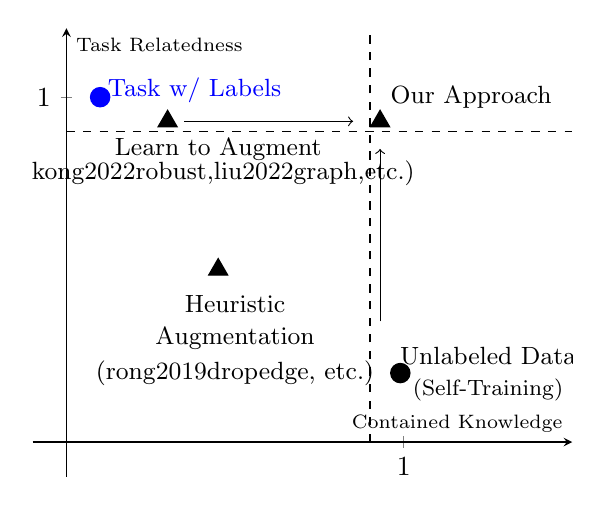
\begin{tikzpicture}
    \begin{axis}
    [
        legend pos= north east,
        axis lines = center,
        domain=-1:2,
        xlabel={\scriptsize Contained Knowledge},
        xmin=-0.1,
        xmax=1.5,
        xtick={0, 1},
        ylabel={\scriptsize Task Relatedness},
        ymin=-0.1,
        ytick={0, 1},
        ymax=1.2,
    ]
    % purple pentagon
    \addplot[only marks, color=black, mark=triangle*, mark size=4pt] coordinates { (0.93,0.93) };
    \node[] at (axis cs: 1.2, 1.0) {\textcolor{black}{\small Our Approach}};

    
    % magenta
    \addplot[only marks, color=black, mark=triangle*,mark size=4pt] coordinates {(0.3,0.93)};
    \node[] at (axis cs: 0.45,0.85) {\textcolor{black}{\small Learn to Augment}};
    \node[] at (axis cs: 0.45,0.78) {\small (\citeauthor{kong2022robust},\citeauthor{liu2022graph},etc.)};
    
    % cyan
    \addplot[only marks, color=black, mark=triangle*,mark size=4pt]
        coordinates {(0.45,0.5) };
    \node[] at (axis cs: 0.5,0.4) {\textcolor{black}{\small Heuristic}};
    \node[] at (axis cs: 0.5,0.3) {\textcolor{black}{\small Augmentation}};
    \node[] at (axis cs: 0.5,0.2) {\textcolor{black}{\small (\citeauthor{rong2019dropedge}, etc.)}};
    
    % red square
    \addplot[only marks, color=blue, mark=*, mark size=3.5pt]
        coordinates {(0.1,1)};
    \node[] at (axis cs: 0.38,1.02) {\textcolor{blue}{\small Task w/ Labels}};

    % color=blue
    \addplot[only marks, color=black, mark=*, mark size=3.5pt]
        coordinates {(0.99,0.2) };
    \node[] at (axis cs: 1.25,0.25) {\textcolor{black}{\small Unlabeled Data}};
    \node[] at (axis cs: 1.25,0.15) {\textcolor{black}{\footnotesize (Self-Training)}};
    
    \draw [dashed] (0.9,0) -- (0.9,1.2);
    \draw [dashed] (0,0.9) -- (1.5,0.9);
    \draw[->](axis cs: 0.35,0.93)--(axis cs: 0.85,0.93);
    \draw[->](axis cs: 0.93,0.35)--(axis cs: 0.93,0.85);
    % \draw[->](unlabeled)--(ours);
    \end{axis}
\end{tikzpicture}}
%     \vspace{-0.2in}
%     \caption{Qualitative relationship of graphs from different data-centric approach on the task closeness and contained knowledge.
%      } 
%     \label{fig: info relationship}
%     \vspace{-0.3in}
% \end{figure}

\section{Additional Related Work on Data-Centric Approach}\label{add:sec:related}
\paragraph{Data Augmentation}
Data augmentation creates new examples with preserved labels but uses no unlabeled data~\citep{shorten2019survey,kashefi2020quantifying,balestriero2022effects}. Examples of heuristic data augmentation techniques include flipping, distorting, and rotating images~\citep{shorten2019survey}, using lexical substitution, inserting words, and shuffling sentences in texts~\citep{kashefi2020quantifying}, and deleting nodes and dropping edges in graphs~\citep{zhao2022graph}. While human knowledge can be used to improve data diversity and reduce over-fitting in heuristic methods, it is difficult to use a single heuristic method to preserve the different labels for different tasks~\citep{balestriero2022effects, cubuk2019autoaugment}. So, automated augmentation~\citep{cubuk2019autoaugment} learned from data to search for the best policy to combine a bunch of predefined heuristic augmentations. Generation models~\citep{antoniou2017data,bowles2018gan,han2022g} create in-class examples. Other learning ideas such as \textsc{FATTEN}~\citep{liu2018feature} and \textsc{GREA}~\citep{liu2022graph} learned to split the latent space for data augmentation. However, learning and augmenting from insufficient labels at the same time may limit the diversity of new examples and cause over-fitting. \method leverages unlabeled data to avoid them.

\paragraph{Relationship between Data-Centric Approaches} 
\begin{wrapfigure}{r}{5.5cm}
\caption{Qualitative relationship of graphs from different data-centric approach on the task relatedness and contained knowledge.}\label{fig: info relationship}
\resizebox{.8\linewidth}{!}{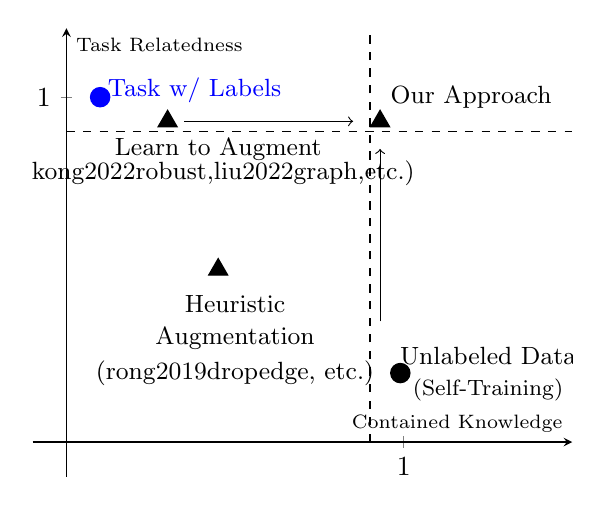
\begin{tikzpicture}
    \begin{axis}
    [
        legend pos= north east,
        axis lines = center,
        domain=-1:2,
        xlabel={\scriptsize Contained Knowledge},
        xmin=-0.1,
        xmax=1.5,
        xtick={0, 1},
        ylabel={\scriptsize Task Relatedness},
        ymin=-0.1,
        ytick={0, 1},
        ymax=1.2,
    ]
    % purple pentagon
    \addplot[only marks, color=black, mark=triangle*, mark size=4pt] coordinates { (0.93,0.93) };
    \node[] at (axis cs: 1.2, 1.0) {\textcolor{black}{\small Our Approach}};

    
    % magenta
    \addplot[only marks, color=black, mark=triangle*,mark size=4pt] coordinates {(0.3,0.93)};
    \node[] at (axis cs: 0.45,0.85) {\textcolor{black}{\small Learn to Augment}};
    \node[] at (axis cs: 0.45,0.78) {\small (\citeauthor{kong2022robust},\citeauthor{liu2022graph},etc.)};
    
    % cyan
    \addplot[only marks, color=black, mark=triangle*,mark size=4pt]
        coordinates {(0.45,0.5) };
    \node[] at (axis cs: 0.5,0.4) {\textcolor{black}{\small Heuristic}};
    \node[] at (axis cs: 0.5,0.3) {\textcolor{black}{\small Augmentation}};
    \node[] at (axis cs: 0.5,0.2) {\textcolor{black}{\small (\citeauthor{rong2019dropedge}, etc.)}};
    
    % red square
    \addplot[only marks, color=blue, mark=*, mark size=3.5pt]
        coordinates {(0.1,1)};
    \node[] at (axis cs: 0.38,1.02) {\textcolor{blue}{\small Task w/ Labels}};

    % color=blue
    \addplot[only marks, color=black, mark=*, mark size=3.5pt]
        coordinates {(0.99,0.2) };
    \node[] at (axis cs: 1.25,0.25) {\textcolor{black}{\small Unlabeled Data}};
    \node[] at (axis cs: 1.25,0.15) {\textcolor{black}{\footnotesize (Self-Training)}};
    
    \draw [dashed] (0.9,0) -- (0.9,1.2);
    \draw [dashed] (0,0.9) -- (1.5,0.9);
    \draw[->](axis cs: 0.35,0.93)--(axis cs: 0.85,0.93);
    \draw[->](axis cs: 0.93,0.35)--(axis cs: 0.93,0.85);
    % \draw[->](unlabeled)--(ours);
    \end{axis}
\end{tikzpicture}}
\end{wrapfigure} 
As presented in~\cref{fig: info relationship}, perturb edges, delete nodes and mask attributes~\citep{rong2019dropedge,trivedianalyzing} for graphs are some heuristic ways for data augmentation. The augmented knowledge from them is mainly controlled by human prior knowledge on the perturbations and it often fails to be close to the task, \ie, random perturbations hardly preserve labels for the augmented graphs. The learning to augment approaches learn from labeled graphs to perturb graph structures~\citep{luo2022automated}, to estimate graphons for different classes~\citep{han2022g}, or to split the latent space for augmentation~\citep{liu2022graph}. Although these approaches could preserve labels for the augmented graphs, they introduce less extra knowledge to improve the model prediction. In summary, graph data augmentation is effective in expanding knowledge for limited labels, but it makes no use of unlabeled graphs. Besides, the diversity and richness of the domain knowledge from augmented graphs are far from that contained in a large number of unlabeled graphs. To learn from unlabeled graphs, data-centric approaches like the self-training is assumed to be useful when the unlabeled and labeled data are from the same source. It is less studied when we have a single unified unlabeled source for different tasks.
% If we assign pseudo-labels for material-related properties to drug-related unlabeled graphs or vice versa, it could negatively impact the model performance. 

\section{Additional Method Details}
\subsection{Upper bounding the mutual information}
In~\cref{eq:upper bound infonce}, we use a leave-one-out variant of InfoNCE ($\I_\text{bound}$) to derive the upper bound of mutual information. We summarize the derivation~\citep{poole2019variational} here.
\begin{equation}\label{eq:add derivation mi upper bound}
    \begin{split}
        \mathcal{I}_1(G^\prime;G) & = \mathbb{E}_{p (G, G^\prime)} \left[ \operatorname{log} \frac{p(G^\prime|G)}{p(G^\prime)} \right] \\
        & = \mathbb{E}_{p (G, G^\prime)} \left[ \operatorname{log} \frac{p(G^\prime|G) q(G^\prime)}{q(G^\prime) p(G^\prime)} \right] \\
        & = \mathbb{E}_{p (G, G^\prime)} \left[ \operatorname{log} \frac{p(G^\prime|G)}{q(G^\prime)} \right] - \operatorname{KL} (p(G^\prime) || q(G^\prime) ) \\
        & \leq \mathbb{E}_{p (G, G^\prime)} \left[ \operatorname{log} \frac{p(G^\prime|G)}{q(G^\prime)} \right]
        % \\ & = \mathbb{E}_{p(G)} \left[\operatorname{KL} (p(G^\prime| G) || q(G^\prime)) \right]
    \end{split}    
\end{equation}
The intractable upper bound is minimized when the variational approximation $q(G^\prime)$ matches the true marginal $p(G^\prime)$~\citep{poole2019variational}. 
% InfoNCE assumes the density ratio is proportional to $\frac{p(G^\prime|G)}{p(G^\prime)}$. 
For each $G_i$, its augmented output $G_i^\prime$, and $M-1$ negative examples with different labels, we could approximate $q(G_i^\prime) = \frac{1}{M-1} \sum_{j \neq i} p(G_i^\prime | G_j)$. So, we have
\begin{equation}
    \begin{split}
        \mathcal{I}_1(G^\prime_i, G_i) 
        & \leq  \operatorname{log} \frac{p(G_i^\prime| G_i)}{\frac{1}{K-1} \sum_{j=1, j\neq i}^M p(G_i^\prime | G_j)}
        \\ & = \operatorname{log} \frac{p(G_i^\prime| G_i)}{\sum_{j=1, j\neq i}^M p(G_i^\prime | G_j)} + \operatorname{log} (M-1)
        % \\ & \leq \operatorname{log} \frac{p(G_i^\prime| G_i)}{\sum_{k=1, k\neq i}^K p(G_i^\prime | G_k)}
        \\ & = \I_\text{bound} (G_i^\prime; G_i) + \text{constant}
    \end{split}
\end{equation}

\subsection{Extraction of Statistical Features on Graphs}\label{add:sec:raw feature}
For each molecule and polymer graph, we concatenate the following vectors or values for statistical feature extraction.
\begin{compactitem}
    \item the sum of the degree in the graph;
    \item the vector indicating the distribution of atom types;
    \item the vector containing the maximum, minimum and mean values of atoms weights in a molecule or polymer;
    \item the vector containing the maximum, minimum, and mean values of bond valence.
\end{compactitem}
For each protein-protein interaction ego-graph in the biology field, we use the sorted vector of node degree distribution in the graph as the statistical features.

\subsection{Technical Details for Graph Data Augmentation with Diffusion Model}\label{add:method:tech}

\paragraph{The Lookup Table from Atom Type to Node Embedding Space}
Given a graph $G$, we assume the node feature matrix on the graph is $\mathbf{X} \in \mathbb{R}^{n \times F_\text{n}}$, where $n$ is the number of nodes. The edge feature matrix is $\mathbf{E} \in \mathbb{R}^{m \times F_\text{e}}$, where $m$ is the number of edges. There are two ways for $G$ to represent the graph structure in practice. We can use either the dense adjacency matrix $\mathbf{A} \in \mathbb{R}^{n \times n}$ or sparse edge index $\mathbf{I}_e \in \mathbb{R}^{2 \times m}$. The diffusion model~\citep{jo2022score} on graphs prefers the former, which is more straightforward for graph generations. The prediction model prefers the latter because of its flexibility, and less computational cost and time. The transformation between two types of graph structure representation takes additional time. Particularly for molecular graphs, the node features used for generation (one-hot encoding of the atom type) and for prediction (see the official package of OGBG~\footnote{\url{https://github.com/snap-stanford/ogb/blob/master/ogb/utils/features.py}} for details) are different, which introduces extra time to process the graph data. For details, we (1) first need to extract discrete node attributes given the atom type and its neighborhoods; (2) we then need to use an embedding table to embed node attributes in a continuous embedding space; (3) the embedding features of nodes with their graph structure are inputted into the graph neural networks to get the latent representation for nodes. The reverse process for data augmentation in \method may need to repeatedly process graph data with steps (1) and (2). It introduces additional time. So, we build up a lookup table to directly map the atom type to the node embedding. To achieve it, we average the node attributes for the same type of node within the batch. We then use the continuous node attributes as weights to average the corresponding node embedding according to the embedding table.

\paragraph{Instantiations of SDE on Graphs} According to~\citet{song2020score}, we use the Variance Exploding (VE) SDE for the diffusion process. Given the minimal noise $\sigma_{\min}$ and the maximal noise $\sigma_{\max}$, the VE SDE is:
\begin{equation}
\mathrm{d} G =\sigma_{\min }\left(\frac{\sigma_{\max }}{\sigma_{\min }}\right)^t \sqrt{2 \log \frac{\sigma_{\max }}{\sigma_{\min }}} \mathrm{d} \mathbf{w}, \quad t \in(0,1]
\end{equation}
% \begin{equation}
% G^{(t)} - G^{(t-1)} = \sqrt{(\sigma^{(t)})^2 - (\sigma^{(t-1)})^2} \cdot \mathbf{z}^{(t-1)}, \quad \quad t=1,\cdots, N_T 
% \end{equation}
% where $\mathbf{z}^{(t)} \sim \mathcal{N} (\mathbf{0}, \mathbf{I})$ 
The perturbation kernel is derived~\citep{song2020score} as:
\begin{equation}
p_{0 t}(G^{(t)} \mid G^{(0)})=\mathcal{N}\left(G^{(t)} ; G^{(0)}, \sigma_{\min }^2\left(\frac{\sigma_{\max }}{\sigma_{\min }}\right)^{2 t} \mathbf{I}\right), \quad t \in(0,1]
\end{equation}

On graphs, we follow~\citet{jo2022score} to separate the perturbation of adjacency matrix and node features:
\begin{equation}
    p_{0 t}(G^{(t)} \mid G^{(0)}) = p_{0 t}(\mathbf{A}^{(t)} \mid \mathbf{A}^{(0)}) p_{0 t}(\mathbf{X}^{(t)} \mid \mathbf{X}^{(0)}).
\end{equation}


\paragraph{The Sampling Algorithm in the Reverse Process for Graph Data Augmentation} We adapt the Predictor-Corrector (PC) samplers for the graph data augmentation in the reverse process. The algorithm is shown in~\cref{alg:diffusion augmentation}.
\begin{algorithm}[H]
   \caption{Diffusion-Based Graph Augmentation with PC Sampling}
   \small
   \label{alg:diffusion augmentation}
   \def\bfX{\mathbf{X}}
   \def\bfz{\mathbf{z}}
   \def\bfI{\mathbf{I}}
   \def\mclN{\mathcal{N}}
\begin{algorithmic}
    % \STATE $\mathbf{z}_0 \sim  \mclN(\mathbf{0}, \bfI)$
    % \STATE $\mathbf{X}^{(D)} \gets \mathbf{X} + \mathbf{z}_0; \quad \mathbf{A}^{(D)} \gets \mathbf{A} + \mathbf{z}_0$
    \STATE {\bfseries Input:} Graph $G$ with node feature $\mathbf{X}$ and adjacency matrix $\mathbf{A}$, the denoising function for node feature $\mathbf{s}_{\mathbf{X}}$ and adjacency matrix $\mathbf{s}_{\mathbf{A}}$, the fine-tune loss $\mathcal{L}_\textbf{aug}$, Lagevin MCMC step size $\beta$,  scaling coefficient $\epsilon_1$
    \STATE $\mathbf{A}^{(D)} \gets \mathbf{A} + \mathbf{z}_A $; \quad $\mathbf{z}_A \sim \mclN(\mathbf{0}, \bfI)$
    \STATE $\mathbf{X}^{(D)} \gets \mathbf{X} + \mathbf{z}_X $; \quad $\mathbf{z}_X \sim \mclN(\mathbf{0}, \bfI)$
    
   \FOR{$t=D-1$ {\bfseries to}  $0$}
    \STATE $\hat{G}_{(t+1)} \sim p_{0 t+1} ( \hat{G}_{(t+1)} |G^{(t+1)}) $ \COMMENT{inner-loop sampling with another PC sampler}
    
    \STATE $ \mathbf{S}_A = \frac{1}{2} \mathbf{s}_{\mathbf{A}}(G^{(t+1)}, t+1) - \frac{1}{2} 
    \alpha \nabla_{\mathbf{A}^{(t)}} \mathcal{L}_\textbf{aug}(\hat{G}_{(t+1)})$
    
    \STATE  $ \mathbf{S}_X = \frac{1}{2} \mathbf{s}_{\mathbf{X}}(G^{(t+1)}, t+1) - \frac{1}{2} 
    \alpha \nabla_{\mathbf{X}^{(t)}} \mathcal{L}_\textbf{aug}(\hat{G}_{(t+1)})$
    
    \STATE $\tilde{\mathbf{A}}^{(t)} \gets \mathbf{A}^{(t+1)} + g(t)^2 \mathbf{S}_A + g(t) \mathbf{z}_A $; \quad $\mathbf{z}_A \sim \mclN(\mathbf{0}, \bfI)$ \COMMENT{Predictor for adjacency matrix}
    \STATE $\tilde{\mathbf{X}}^{(t)} \gets \mathbf{X}^{(t+1)} +  g(t)^2 \mathbf{S}_X  + g(t) \mathbf{z}_X $; \quad $\mathbf{z}_X \sim \mclN(\mathbf{0}, \bfI)$ \COMMENT{Predictor for node features}
    \STATE $\mathbf{A}^{(t)} \gets \tilde{\mathbf{A}}^{(t)} + \frac{\beta}{2} \mathbf{S}_A + \epsilon_1 \sqrt{\beta} \mathbf{z}_A $; \quad $\mathbf{z}_A \sim \mclN(\mathbf{0}, \bfI)$ \COMMENT{Corrector for adjacency matrix}
    \STATE $\mathbf{X}^{(t)} \gets \tilde{\mathbf{X}}^{(t)} + \frac{\beta}{2} \mathbf{S}_X  + \epsilon_1 \sqrt{\beta} \mathbf{z}_X $; \quad $\mathbf{z}_X \sim \mclN(\mathbf{0}, \bfI)$ \COMMENT{Corrector for node features}

     % \FOR{$j=1$ {\bfseries to} $M$}
     %    \STATE $z \sim {N}(0, I)$
     %    \STATE{$G_{i} \gets G_{i} + \epsilon_i S(G_{i}, \sigma_{i}) + \sqrt{2\epsilon_i} z$}
     % \ENDFOR
   \ENDFOR
   \STATE {return} $G^\prime  = ( \mathbf{A}^{(0)}, \mathbf{X}^{(0)})$
\end{algorithmic}
\end{algorithm}




\section{Additional Experiments Set-ups}\label{sec: add exp setups}
We perform experiments on 15 datasets, including eight classification and seven regression tasks from chemistry, material science, and biology. We use Area under the ROC curve (AUC) for classification performance and mean absolute error (MAE) for regression.
\subsection{Molecule Classification and Regression Tasks}
Seven molecule classification and three molecule regression tasks are from open graph benchmark~\citep{hu2020open}. They were originally collected by MoleculeNet~\citep{wu2018moleculenet} and used to predict molecule properties. They include (1) inhibition to HIV virus replication in \hiv, (2) toxicological properties of 617 types in \toxcast, (3) toxicity measurements such as nuclear receptors and stress response in \toxt, (4) blood–brain barrier permeability in \bbbp, (5) inhibition to human $\beta$-secretase 1 in \bace, (6) FDA approval status or failed clinical trial in \clintox, (7) having drug side effects of 27 system organ classes in \sider, (8) predicting the property of lipophilicity in \lipo, (9) predicting the water solubility ($\log$ solubility in mols per litre) from chemical structures in \esol, (10) predicting the hydration free energy of molecules in water in \freesolv.
For all molecule datasets, we use the scaffold splitting procedure as the open graph benchmark adopted \citep{hu2020open}. It attempts to separate structurally different molecules into different subsets, which provides a more realistic estimate of model performance in experiments~\citep{wu2018moleculenet}.

\subsection{Polymer Regression Tasks}
Four polymer regression tasks include \glass, \melting, \thermal, and \oxygen. They are used to predict different polymer properties such as \emph{glass transition temperature} ($^\circ$C), \emph{melting temperature} ($^\circ$C), \emph{thermal conductivity} (W/mK) and \emph{oxygen permeability} (Barrer). \glass and \melting are collected from PolyInfo, which is the largest web-based polymer database \citep{otsuka2011polyinfo}. The \thermal dataset is from molecular dynamics simulation and is an extension from the dataset used in~\citep{ma2022machine}. The \oxygen dataset is created from the Membrane Society of Australasia portal,
consisting of a variety of gas permeability data \citep{thornton2012polymer}. Since a polymer is built from repeated units, researchers often use a single unit graph with polymerization points as polymer graphs to predict properties. Different from molecular graphs, two polymerization points are two special nodes (see ``$*$'' in \cref{fig:implementation}), indicating the polymerization of monomers \citep{cormack2004molecularly}. For all the polymer tasks, we randomly split by 60\%/10\%/30\% for training, validation, and test.

% Particularly, \textbf{tasks used in \cref{fig:compare gnn runs}} are hiv (\hiv), bace (\bace), bbbp (\bbbp), clintox (\clintox), sider (\sider), tox21 (\toxt), toxcast (\toxcast), oxygen (\oxygen), melting (\melting), and glass (\glass).

\subsection{Protein Classification Task}
An additional task is protein function prediction using protein-protein interaction graphs~\citep{hu2019strategies}. A node is a protein without attributes, an edge is a relation type between two proteins such as co-expression and co-occurrence. In our \method, we treat all the relations as the undirected edge without attributes.


\subsection{Baselines and Implementation}
When implementing \gin~\citep{xu2018powerful}, we tune its hyper-parameters for different tasks with an early stop on the validation set. We generally implement pre-training baselines following their own setting. For molecule and polymer property prediction and protein function prediction, the pre-trained \gin models with self-supervised tasks such as \edgepred, \attrmask, \contextpred in~\citep{hu2019strategies}, \infomax~\citep{velickovic2019deep} are available. So we directly use them. For other self-supervised methods, we implement their codes with default hyper-parameters. Following their settings, we use 2M ZINC15~\citep{sterling2015zinc} to pre-train \gin models for molecule and polymer property prediction. We use 306K unlabeled protein-protein interaction ego-networks~\citep{hu2019strategies} to pre-train the \gin for the downstream protein function property prediction. For self-training with real unlabeled graphs and \infograph~\citep{sun2019infograph}, we use 113K QM9~\citep{ramakrishnan2014quantum}. For self-training with generated unlabeled graphs, we train the diffusion model~\citep{jo2022score} on the real QM9 dataset and then produce the same number of generated unlabeled graphs. To train the diffusion model in our \method, we also use QM9~\citep{ramakrishnan2014quantum}.

% \begin{table}[t]
\centering
\footnotesize
\setlength{\tabcolsep}{4pt} 
\begin{tabular}{lccccc}
\toprule
 & \makecell{Visual\\Context} & \makecell{\#Dialog} & \makecell{Avg. \\\#Turn} & \makecell{Avg. Utt. \\Length} & \makecell{\#Tokens}\\
\midrule 
BST~\citep{smith2020can} & \xmark & 7K & 11.2 & 13.6 & 1M\\
ConvAI2~\citep{dinan2020second} & \xmark & 20K & 13.9 & 9.9 & 2.7M \\
ED~\citep{rashkin2018towards} & \xmark & 25K & 4.3 & 13.7 & 1.5M \\
WOW~\citep{dinan2018wizard} & \xmark & 22K & 9.1 & 16.4 & 3.3M\\
WOI~\citep{komeili2021internet} & \xmark & 9.5K & 10.9 & 13.9 & 1.4M\\
SODA~\citep{kim2022soda} & \xmark & 1.5M & 7.6 & 16.1 & 183M\\
ImageChat~\citep{shuster2018image} & \cmark & 100K & 3.0 & 9.7 & 2.9M \\
OVD2.0~\citep{wang2021openvidial} & \cmark & 116K & \textbf{48.7} & 6.3  & 35.6M\\
MMD~\citep{feng2022mmdialog} & \cmark & 1M & 4.5 & 15.9 & 71.5M \\
\midrule
\datasetName & \cmark & \textbf{18M} & 3.0 & \textbf{19.7} & \textbf{1.06B}\\
\bottomrule
\end{tabular}
\caption {
Statistics of \datasetNameNoEmoji compared to other open-domain dialogue and visually grounded dialogue dataset. \textit{Utt.} stands for utterance.
}
\label{tab:dataset_statistics}
\end{table}


\section{Additional Experiment Analysis}
% \section{Additional Experiments Results and Analysis}


% \definecolor{LightCyan}{rgb}{0.88,1,1}
% \definecolor{negative}{gray}{0.92}
% \begin{table*}[ht!]
%     \renewcommand{\arraystretch}{1.1}
%     \renewcommand{\tabcolsep}{1.5mm}
%     \caption{\small More results {Mean\scriptsize(Std)} on regression tasks. The best mean is \textbf{bonded}. The best baseline is \underline{underlined}. Results are \colorbox{negative}{highlighted} if unlabeled graphs bring significant negative impacts compared to \gin. The MAE for \thermal is scaled $\times$ 100. }
%     \centering
%     \begin{adjustbox}{width=0.98\textwidth}
%     \begin{tabular}{llccccccc}
%     %%%%%%%%%%%%%%%%% regression results
%     \toprule
%     \multicolumn{2}{c}{} & \multicolumn{3}{c}{{Molecule Regression: RMSE $\downarrow$}} & \multicolumn{4}{c}{{Polymer Regression: RMSE $\downarrow$}} \\
%     \cmidrule[0.4pt](lr){3-5} \cmidrule[0.4pt](lr){6-9}
%     & & \lipo & \esol & \freesolv & \glass & \melting & \thermal & \oxygen\\
%     \multicolumn{2}{c}{\# Training Graphs} & 3,360 & 902 & 513 & 4,303 & 2,189 & 455 & 356 \\
%     \midrule
    
%     & \gin & 0.707{\scriptsize (0.022)} & 1.002{\scriptsize (0.032)} & {\scriptsize (X)} 
%     & X {\scriptsize (XX )} & XX {\scriptsize (XX)} & XX {\scriptsize (XXX)} & XXX{\scriptsize (XXX)}
%     \\

%     \midrule
%     \multirow{7}{*}{\rotatebox{90}{\textit{\fontsize{8pt}{8pt} Self-Supervised}}}
    
%     & \edgepred 
%     & 0.773{\scriptsize (0.012)} & X{\scriptsize (XX )} & {\scriptsize (X)} 
%     & X {\scriptsize (XX )} & XX {\scriptsize (XX)} & XX {\scriptsize (XXX)} & XXX{\scriptsize (XXX)} \\
%     & \attrmask 
%     &  0.757{\scriptsize (0.011)} & X{\scriptsize (XX )} & {\scriptsize (X)} 
%     & X {\scriptsize (XX )} & XX {\scriptsize (XX)} & XX {\scriptsize (XXX)} & XXX{\scriptsize (XXX)} \\
%     & \contextpred 
%     & 0.783{\scriptsize (0.013)} & X{\scriptsize (XX )} & {\scriptsize (X)} 
%     & X {\scriptsize (XX )} & XX {\scriptsize (XX)} & XX {\scriptsize (XXX)} & XXX{\scriptsize (XXX)}\\
%     & \infomax 
%     &  0.752{\scriptsize (0.013)} & X{\scriptsize (XX )} & {\scriptsize (X)} 
%     & X {\scriptsize (XX )} & XX {\scriptsize (XX)} & XX {\scriptsize (XXX)} & XXX{\scriptsize (XXX)} \\
%     & \joao 
%     & 0.770 {\scriptsize (0.010)} & X{\scriptsize (XX )} & {\scriptsize (X)} 
%     & X {\scriptsize (XX )} & XX {\scriptsize (XX)} & XX {\scriptsize (XXX)} & XXX{\scriptsize (XXX)}\\
%     & \graphlog 
%     &  0.759{\scriptsize (0.012)} & X{\scriptsize (XX )} & {\scriptsize (X)} 
%     & X {\scriptsize (XX )} & XX {\scriptsize (XX)} & XX {\scriptsize (XXX)} & XXX{\scriptsize (XXX)} \\
%     & \dsla 
%     &  0.731 {\scriptsize (0.006)} & X{\scriptsize (XX )} & {\scriptsize (X)} 
%     & X {\scriptsize (XX )} & XX {\scriptsize (XX)} & XX {\scriptsize (XXX)} & XXX{\scriptsize (XXX)} \\

%     \midrule
%     \multirow{3}{*}{\rotatebox{90}{\textit{\fontsize{8pt}{8pt} Semi-SL}}}
%     & \infograph 
%     &  0.969{\scriptsize (0.107)} & X{\scriptsize (XX )} & {\scriptsize (X)} 
%     & X {\scriptsize (XX )} & XX {\scriptsize (XX)} & XX {\scriptsize (XXX)} & XXX{\scriptsize (XXX)}  \\
    
%     & \streal 
%     &  0.696{\scriptsize (0.008)} & 1.021{\scriptsize (0.106)} & {\scriptsize (X)} 
%     & X {\scriptsize (XX )} & XX {\scriptsize (XX)} & XX {\scriptsize (XXX)} & XXX{\scriptsize (XXX)} \\
%     & \stgen &
%      0.698{\scriptsize (0.029)} & 0.928{\scriptsize (0.116)} & {\scriptsize (X)} & X {\scriptsize (XX )} & XX {\scriptsize (XX)} & XX {\scriptsize (XXX)} & XXX{\scriptsize (XXX)}\\
%     \midrule
%     \multirow{2}{*}{\rotatebox{90}{\textit{\fontsize{8pt}{8pt} GDA}}} 
    
%     & \flag & 0.693{\scriptsize (0.006)} & X{\scriptsize (XX )} & {\scriptsize (X)} & X {\scriptsize (XX )} & XX {\scriptsize (XX)} & XX {\scriptsize (XXX)} & XXX{\scriptsize (XXX)} \\
%     & \grea & 0.753{\scriptsize (0.038)} & X{\scriptsize (XX )} & {\scriptsize (X)} & X {\scriptsize (XX )} & XX {\scriptsize (XX)} & XX {\scriptsize (XXX)} & XXX{\scriptsize (XXX)}\\

%     \midrule
%     & \method~(Ours)  0.683{\scriptsize (0.014)} & X{\scriptsize (XX )} & {\scriptsize (X)} 
%     & X {\scriptsize (XX )} & XX {\scriptsize (XX)} & XX {\scriptsize (XXX)} & XXX{\scriptsize (XXX)} \\
%     \bottomrule
%     \end{tabular}
%     \end{adjustbox}
%     \vspace{-0.1in}
%     \label{add:tab:more reg results}
% \end{table*}

\subsection{The Power of Diffusion Model to Learn from Unlabeled Graphs}
In~\cref{tab:ablation finetune}, when we replace the 133K QM9 with the 249K ZINC~\citep{jo2022score} to train the diffusion model, which nearly doubles the size of the unlabeled graphs and includes more atom types, we do not observe any additional improvement, and in some cases, even worse performance. It is possible because of the constraint of the current diffusion model's capacity to model the data distribution for a much larger number of more complex graphs. It encourages powerful generative models in the future, which could be directly used to benefit predictive models under the proposed framework.

% Appendix here

% \input{figures/math_fig.tex}
\end{document}
